%%%%%%%%%%%%%%%%%%%%%%%%%%%%%%%%%%%%% 
%% LE2I beamer template
%% Guillaume Lemaitre, October 2014
%%%%%%%%%%%%%%%%%%%%%%%%%%%%%%%%%%%%% 

\documentclass{beamer}

\usepackage[utf8]{inputenc}
\usepackage[T1]{fontenc} 
\usetheme{le2i} 

%% The amssymb package provides various useful mathematical symbols
\usepackage{amssymb}
%% The amsthm package provides extended theorem environments
\usepackage{amsthm}
%% amsmath for math environment
\usepackage{amsmath}

\DeclareMathOperator*{\argmin}{arg\,min}
\DeclareMathOperator*{\argmax}{arg\,max}
\DeclareMathOperator*{\sign}{sign}

%% Text packages
\usepackage[nolist]{acronym}

%% figure package
\usepackage{epsf,graphicx}
\usepackage{epstopdf}
\usepackage{subfigure}
\usepackage{transparent}

%% In order to draw some graphs
\usepackage{tikz,xifthen}
\usepackage{tikz-qtree}
\usepackage{adjustbox}
\usetikzlibrary{decorations.pathmorphing}
\usetikzlibrary{fit}
\usetikzlibrary{backgrounds}
\usetikzlibrary{shapes,arrows,shadows}
\usetikzlibrary{calc,decorations.pathreplacing,decorations.markings,positioning}
\usetikzlibrary{snakes,decorations.text,shapes,patterns}
% \usepackage{scalefnt,lmodern,booktabs}

%% Package for cross and tick symbols
\usepackage{pifont}
\newcommand{\tick}{\color{green!60!black!80}\ding{51}}
\newcommand{\cross}{\color{red!60!black!80}\ding{55}}

\setbeamercovered{transparent}
\resetcounteronoverlays{subfigure}

\usepackage{multirow}
\usepackage{biblatex}
\addbibresource{bibtex.bib}

\title{\Large{Breast Ultrasound Image Segmentation: an optimization approach based on super-pixels and high-level descriptors}}
\author{\scriptsize{Joan Massich\\ \texttt{joan.massich@u-bourgogne.fr}}}
\date{\scriptsize{Quality Control by Artificial Vision \\ 4\textsuperscript{th} June 2015}}

\institute{Universit\'e de Bourgogne} 

\newenvironment<>{redblock}[1]{%
  \begin{actionenv}#2%
    \def\insertblocktitle{#1}%
    \par%
    \mode<presentation>{%
      \setbeamercolor{block title}{fg=nicewhite,bg=red!75!black}
      \setbeamercolor{block body}{fg=niceblack,bg=red!20}
    }%
    \usebeamertemplate{block begin}}
  {\par\usebeamertemplate{block end}\end{actionenv}}

\newenvironment<>{greenblock}[1]{%
  \begin{actionenv}#2%
    \def\insertblocktitle{#1}%
    \par%
    \mode<presentation>{%
      \setbeamercolor{block title}{fg=nicewhite,bg=green!40!black}
      \setbeamercolor{block body}{fg=niceblack,bg=green!20}
    }%
    \usebeamertemplate{block begin}}
  {\par\usebeamertemplate{block end}\end{actionenv}}

%% Uncomment if you want to avoid thousand of bullet inside the menu
% \usepackage{etoolbox}
% \makeatletter
% \patchcmd{\slideentry}{\advance\beamer@xpos by1\relax}{}{}{}
% \def\beamer@subsectionentry#1#2#3#4#5{\advance\beamer@xpos by1\relax}%
% \makeatother

\begin{document}

\graphicspath{{images/generalFigures/}}

% Show the title page
\begin{frame}
  \titlepage
\end{frame}

% % Show the table of contents
% \begin{frame}
%   \tableofcontents[sectionstyle=show,subsectionstyle=show,subsubsectionstyle=hide]
% \end{frame}

\graphicspath{{images/generalFigures/}, {images/word_cloud/}}

\begin{frame}[plain]{}
  \begin{beamercolorbox}[wd=\paperwidth,ht=\paperheight]{frametitle}
    \begin{tikzpicture}
      \fill[azulunam, opacity=1] (0, 0) rectangle(100, 100);
      \node [anchor=center] (cloud) at 
        (0.5\paperwidth, 0.5\paperheight)
        {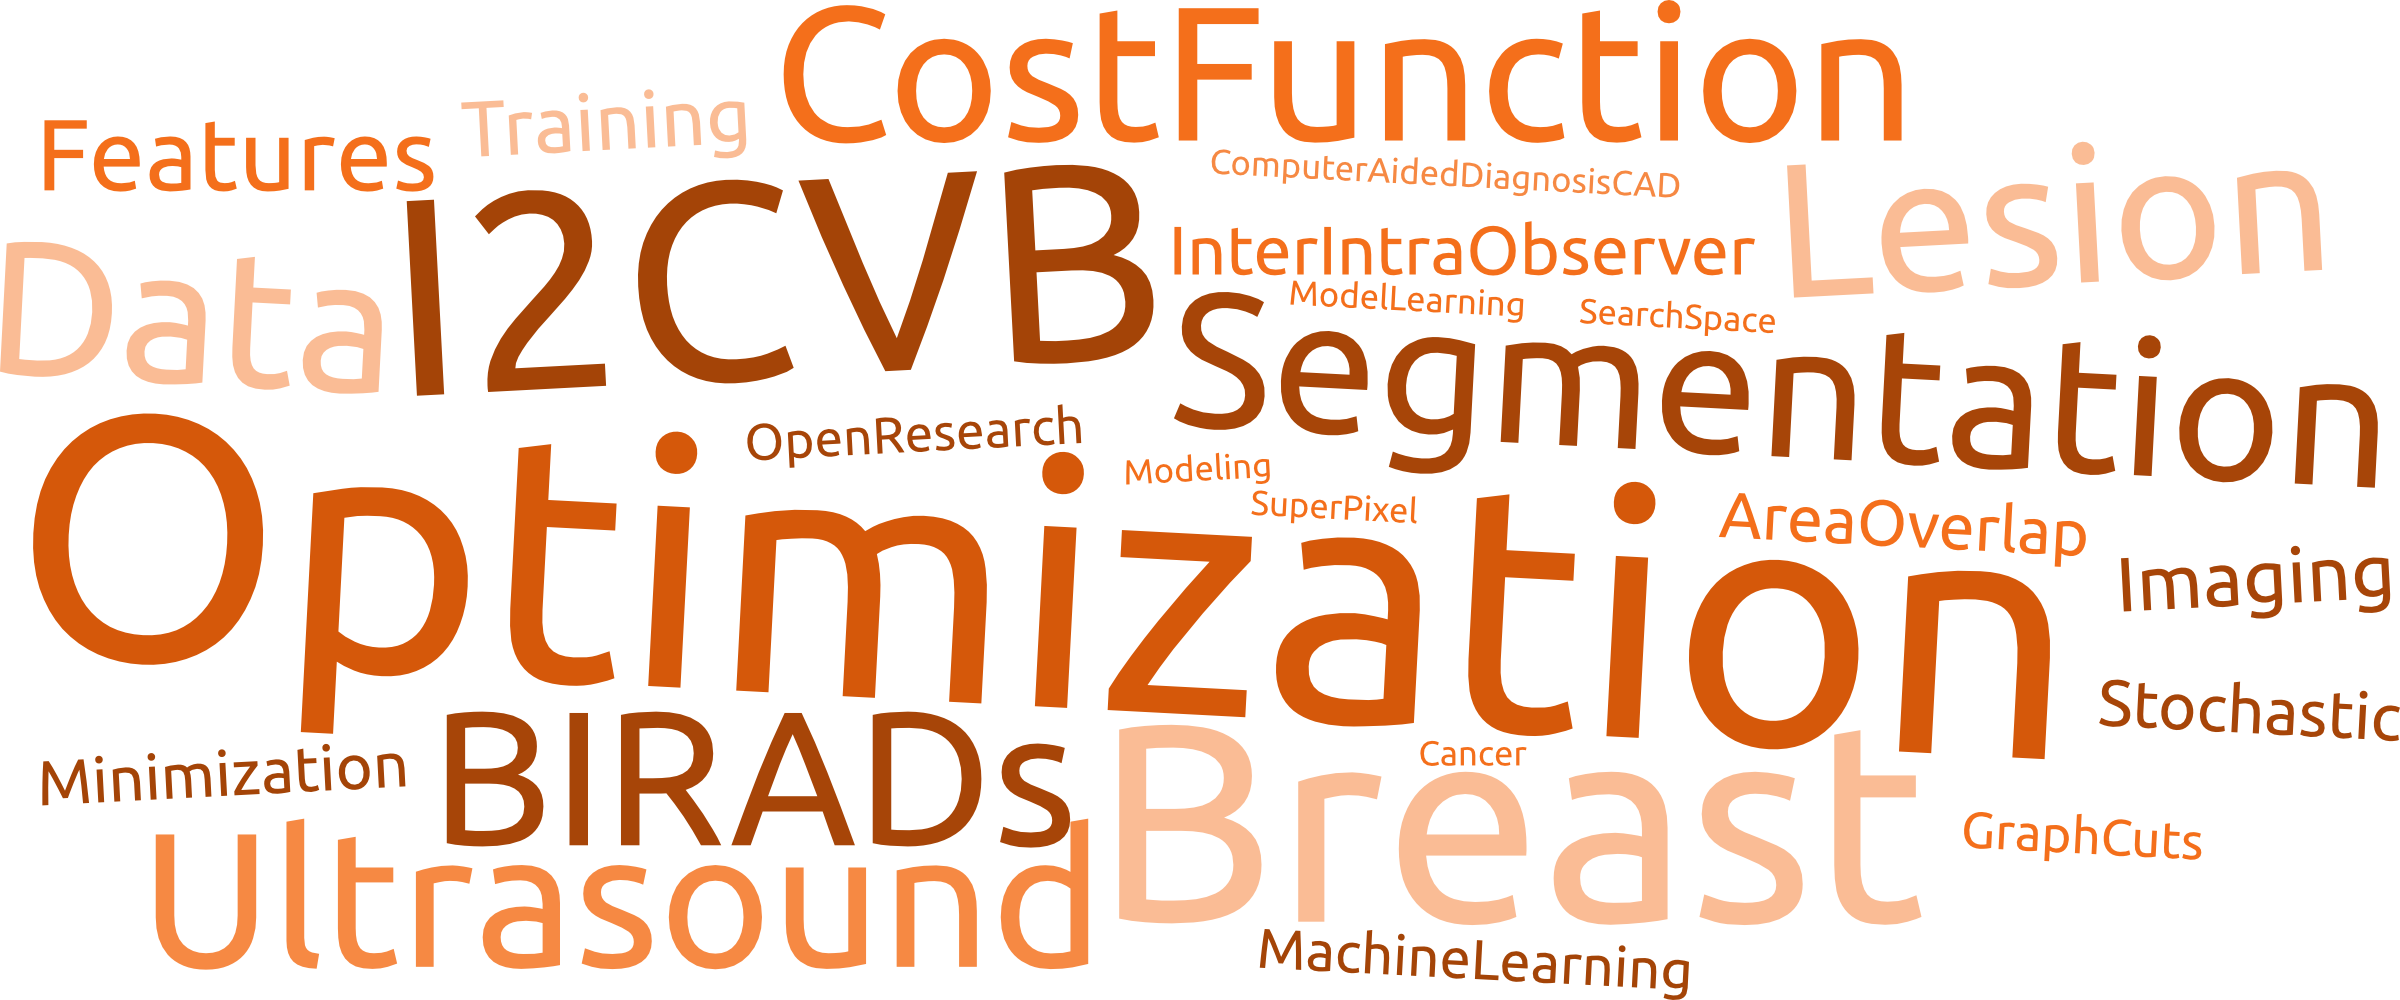
\includegraphics[width=.95\paperwidth]{orange_mix.png}};
    \end{tikzpicture}
  \end{beamercolorbox}
  % 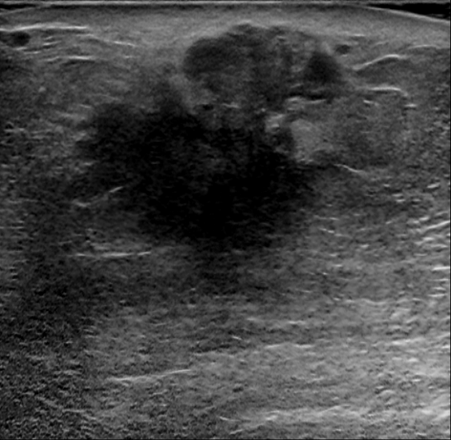
\includegraphics[trim=0 6 0 0,clip,height=.65\textheight]{a110105_094.png}~
\end{frame}


\begin{frame}[plain]{}
  \begin{beamercolorbox}[wd=\paperwidth,ht=\paperheight]{frametitle}
    \begin{tikzpicture}
      \fill[azulunam, opacity=1] (0, 0) rectangle(100, 100);
      \node [anchor=center] (cloud) at 
        (0.5\paperwidth, 0.5\paperheight)
        {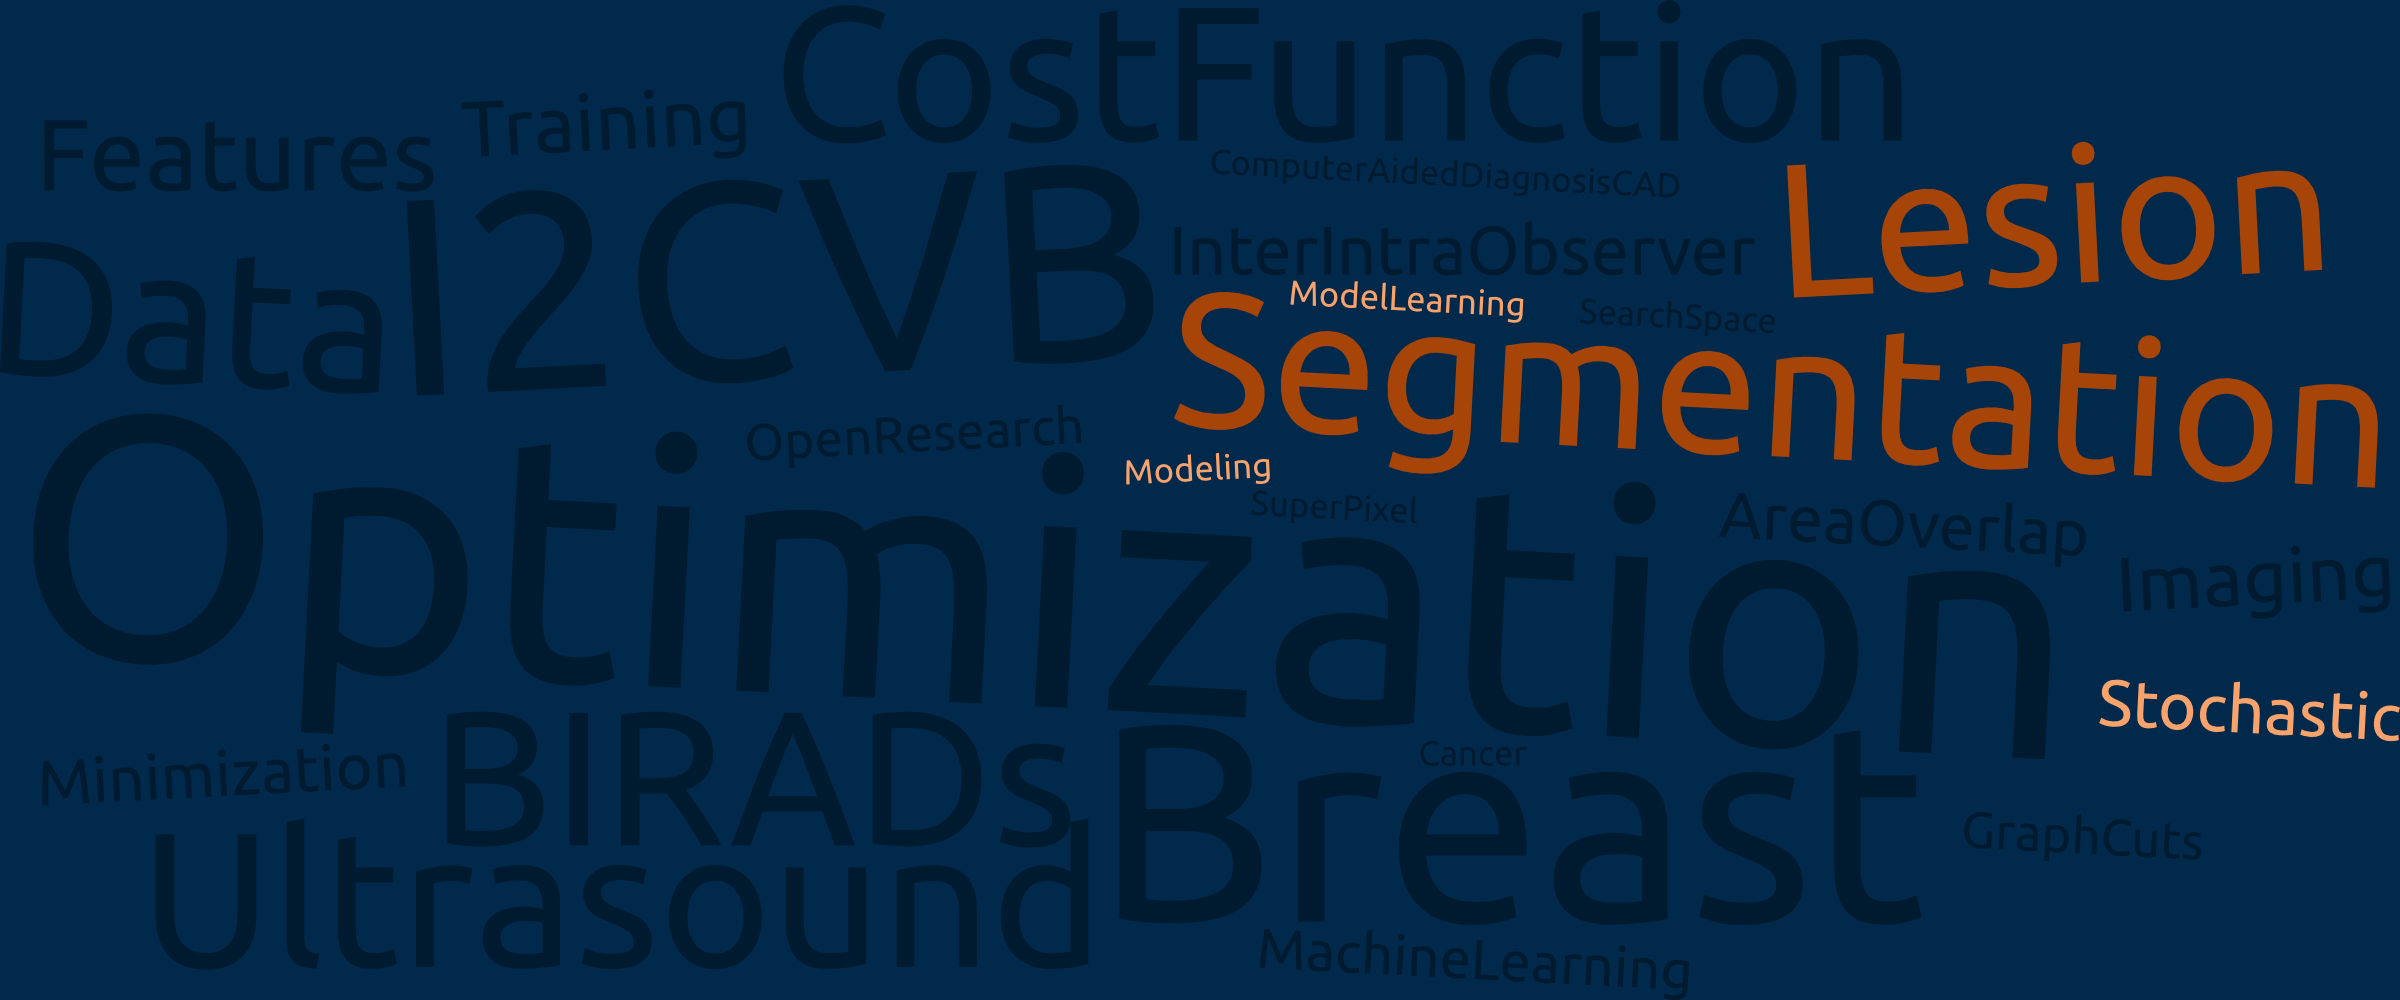
\includegraphics[width=.95\paperwidth]{highlight_prelude.png}};
    \end{tikzpicture}
  \end{beamercolorbox}
  % 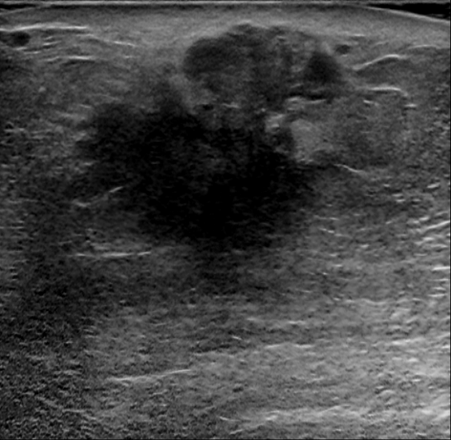
\includegraphics[trim=0 6 0 0,clip,height=.65\textheight]{a110105_094.png}~
\end{frame}

\begin{frame}[plain]\frametitle{Breast Lesion Segmentation in US images}
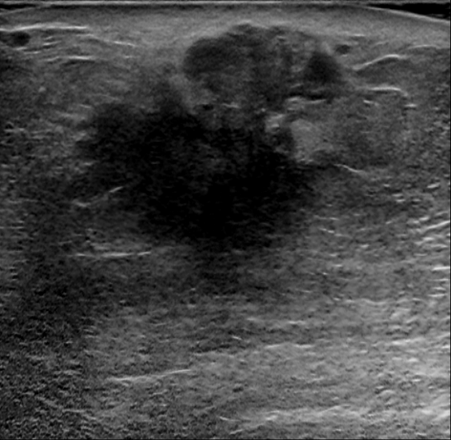
\includegraphics[trim=0 6 0 0,clip,height=.40\paperwidth]{a110105_094.png}~
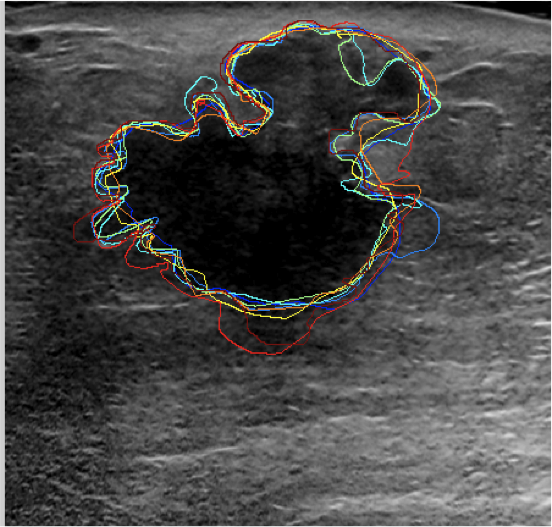
\includegraphics[trim=6 0 0 0,clip,height=.40\paperwidth]{segment.png}
\end{frame}



\begin{frame}
  \begin{beamercolorbox}[wd=\paperwidth,ht=\paperheight]{frametitle}
    \begin{tikzpicture}
      \fill[nicewhite, opacity=1] (0, 0) rectangle(1, 1);
      \node [anchor=center] (cloud) at 
        (0.5\paperwidth, 0.5\paperheight)
        {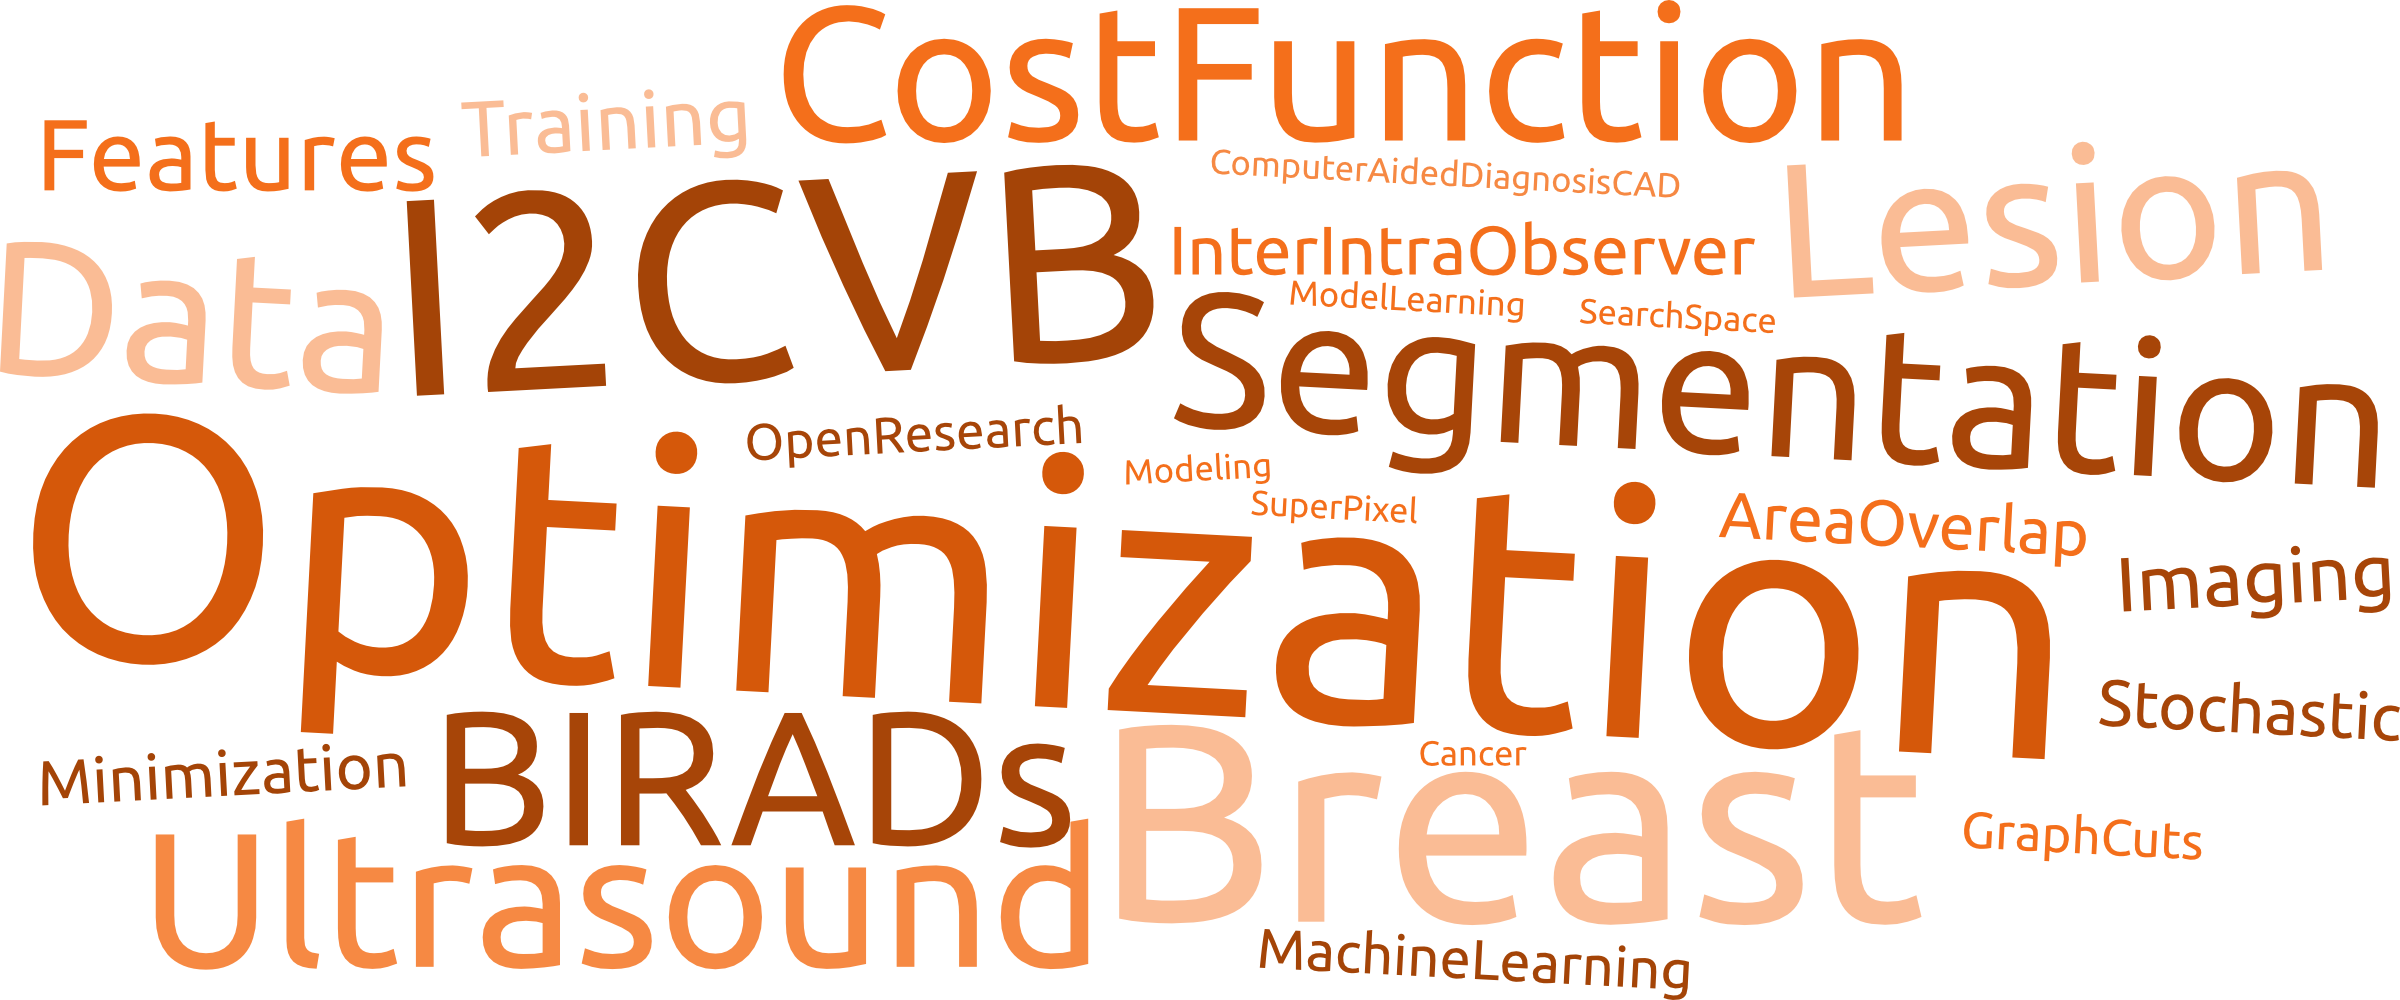
\includegraphics[width=.95\paperwidth]{orange_mix.png}};
    \end{tikzpicture}
  \end{beamercolorbox}
\end{frame}


\begin{frame}
  \begin{beamercolorbox}[wd=\paperwidth,ht=\paperheight]{frametitle}
    \begin{tikzpicture}
      \fill[nicewhite, opacity=1] (0, 0) rectangle(1, 1);
      \node [anchor=center] (cloud) at 
        (0.5\paperwidth, 0.5\paperheight)
        {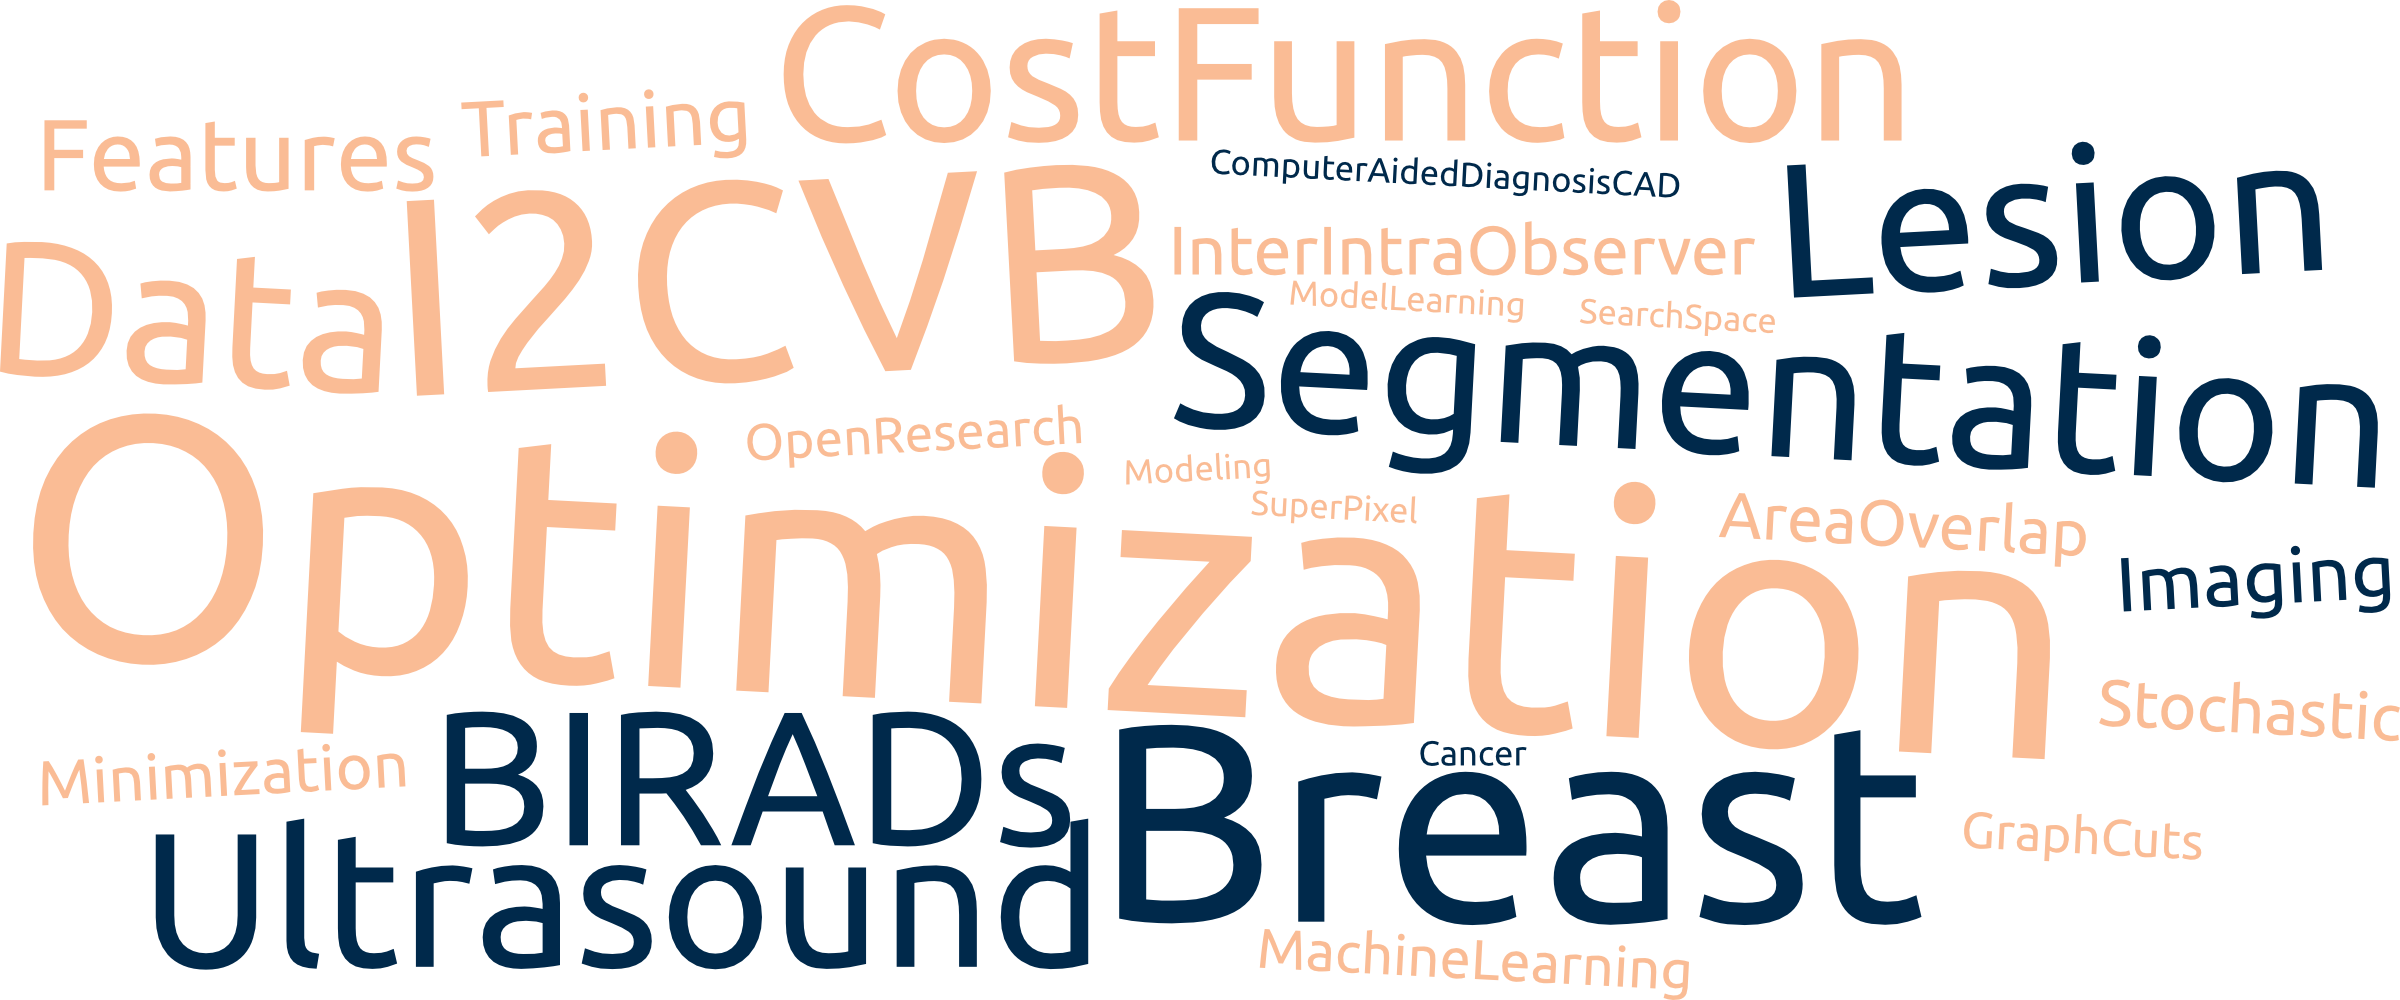
\includegraphics[width=.95\paperwidth]{intro.png}};
    \end{tikzpicture}
  \end{beamercolorbox}
\end{frame}


\begin{frame}
  \begin{beamercolorbox}[wd=\paperwidth,ht=\paperheight]{frametitle}
    \begin{tikzpicture}
      \fill[nicewhite, opacity=1] (0, 0) rectangle(1, 1);
      \node [anchor=center] (cloud) at 
        (0.5\paperwidth, 0.5\paperheight)
        {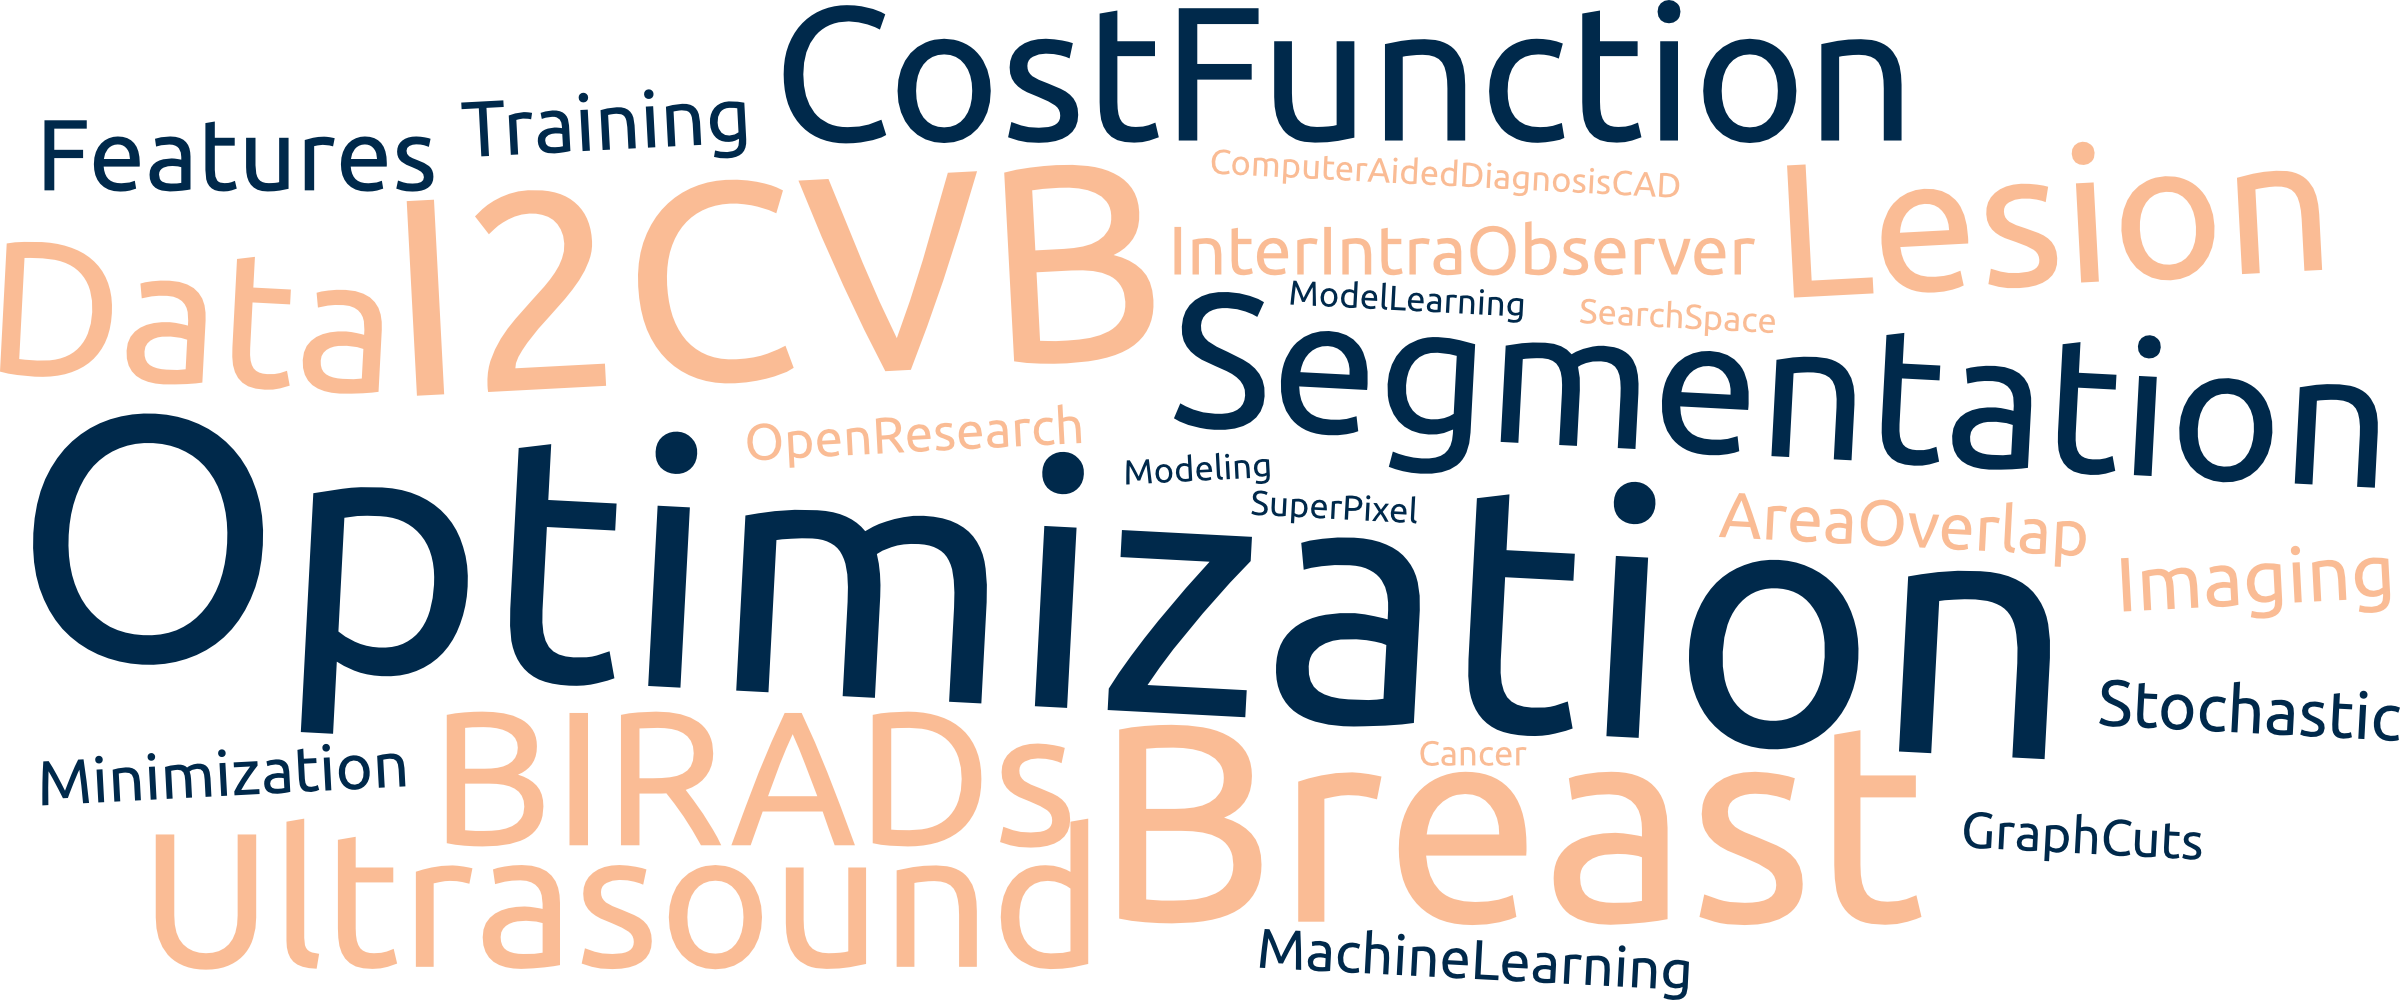
\includegraphics[width=.95\paperwidth]{method.png}};
    \end{tikzpicture}
  \end{beamercolorbox}
\end{frame}

\begin{frame}
  \begin{beamercolorbox}[wd=\paperwidth,ht=\paperheight]{frametitle}
    \begin{tikzpicture}
      \fill[nicewhite, opacity=1] (0, 0) rectangle(1, 1);
      \node [anchor=center] (cloud) at 
        (0.5\paperwidth, 0.5\paperheight)
        {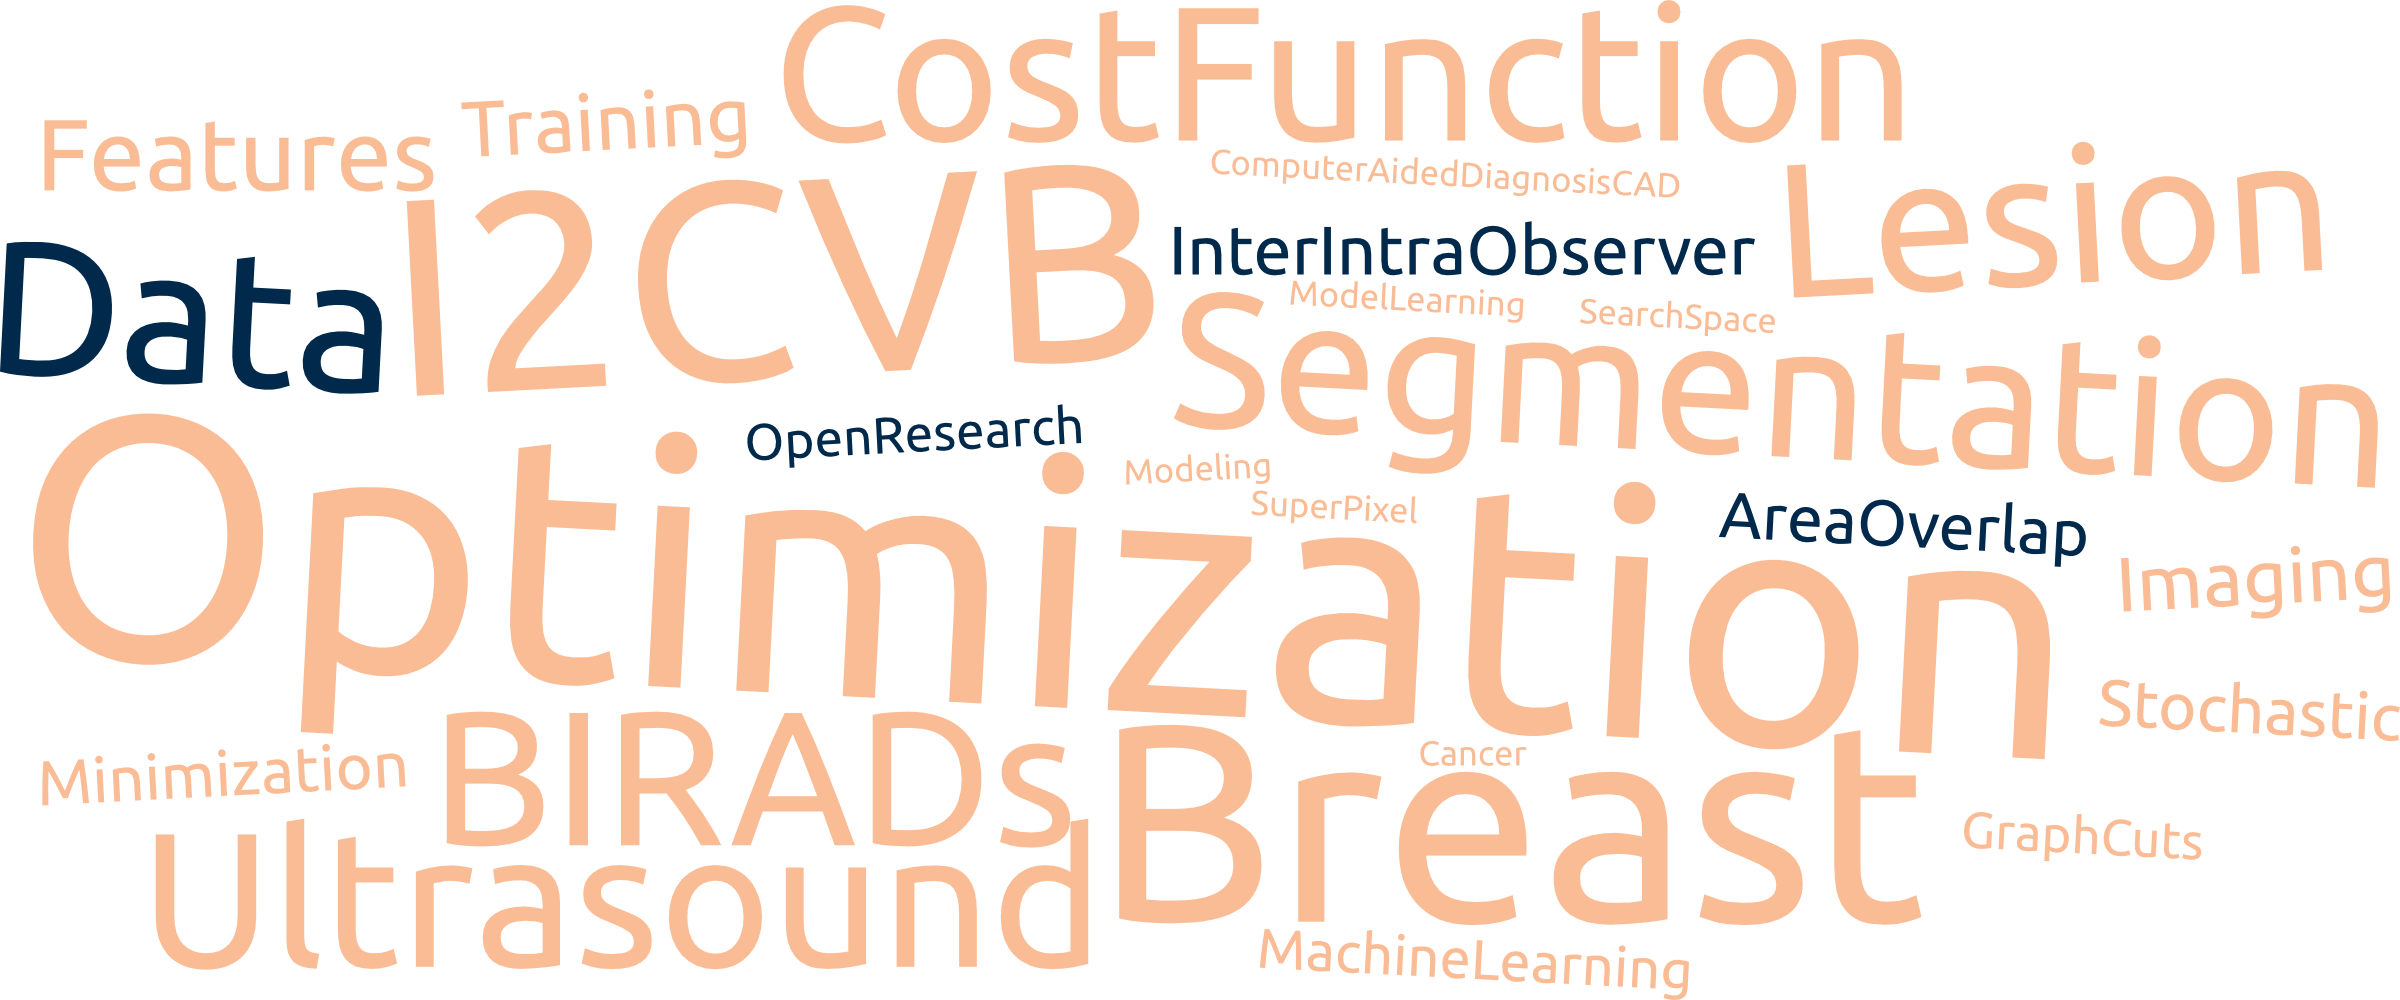
\includegraphics[width=.95\paperwidth]{results.png}};
    \end{tikzpicture}
  \end{beamercolorbox}
\end{frame}

\section{Introduction}
\graphicspath{{chapters/introduction/figures/}}


\subsection{Motivations}

\begin{frame}{Motivations}
  % \frametitle{Introduction}
  % \framesubtitle{Motivations}
  \begin{block}{\small Statistics}
    \begin{figure}%
      \centering
      \hspace*{\fill}%
      \subfigure[][\tiny \# of cancer cases]{%
        \label{fig:stat1a}%
          \includegraphics[width=.45\textwidth]{./images/statistics/repartitionCancerIncidence.png}}%
      \hfill%
      \subfigure[][\tiny \# of cancer deaths]{%
        \label{fig:stat1b}%
          \includegraphics[width=.45\textwidth]{./images/statistics/repartitionCancerDeaths.png}}%
        \hspace*{\fill}%
      \label{fig:stat1}%
    \end{figure}
  \end{block}
  \begin{block}{\small Implications}\footnotesize
    \begin{itemize}
      \item 1.4 million cases per year
      \item 10.9\% of diagnosed cancers
      \item 5\textsuperscript{th} cause of cancer death
      \item 1\textsuperscript{th} cause of cancer death (females)
    \end{itemize}
  \end{block}
\end{frame}

\subsection{Screening}

\begin{frame}{Breast Imaging}
  % \frametitle{Introduction}
  % \framesubtitle{Screening}
  \begin{block}{\small Ultra-Sound(US) distinguishable lesion, shielded under Digital Mammography(DM)}\footnotesize
    \begin{figure}%
      \centering
      \hspace*{\fill}%
      \subfigure[][\tiny DM]{%
        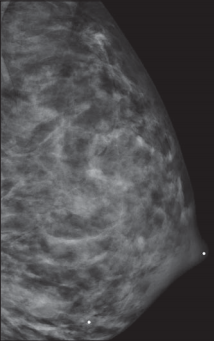
\includegraphics[trim = 0 0 0 20, clip,height=3.3cm]{mamo-us1.png}
        \label{fig:shielda}%
      \hfill%
      \subfigure[][\tiny DM, Region of Interest (ROI) ]{%
        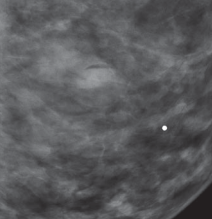
\includegraphics[trim = 0 0 0 20, clip,height=3.3cm]{mamo-us2.png}
        \label{fig:shieldb}%
      \hfill%
      \subfigure[][\tiny Breast Ultra-Sound(BUS), ROI]{%
        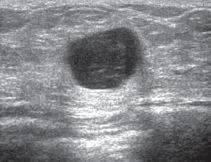
\includegraphics[trim = 10 20 10 0, clip,height=3.3cm]{mamo-us3.png}
        \label{fig:shieldc}%
        \hspace*{\fill}%
      \label{fig:shield}%
    \end{figure}
  \end{block}

  \begin{block}{\small US imaging as adjunct image modality}\footnotesize
    \begin{itemize}
    \item Most common adjunct image modality
    \item Ability to discern solid lesions typologies
    \end{itemize}
  \end{block}

\end{frame}

\subsection{Image formation, limitations and imaging perspectives}
\begin{frame}\frametitle{Breast structures and appearance under US screening}
\begin{columns}
\begin{column}{.48\textwidth}\vspace{-17pt}%\hspace{-1cm}
\begin{figure}\centering
\begin{tikzpicture}[scale=.5]
\begin{scriptsize}
	\tikzset{dot/.style={circle,draw=black,inner sep=0mm,minimum size=4pt}}
    \node[anchor=south west,inner sep=0] at (.2,.2) {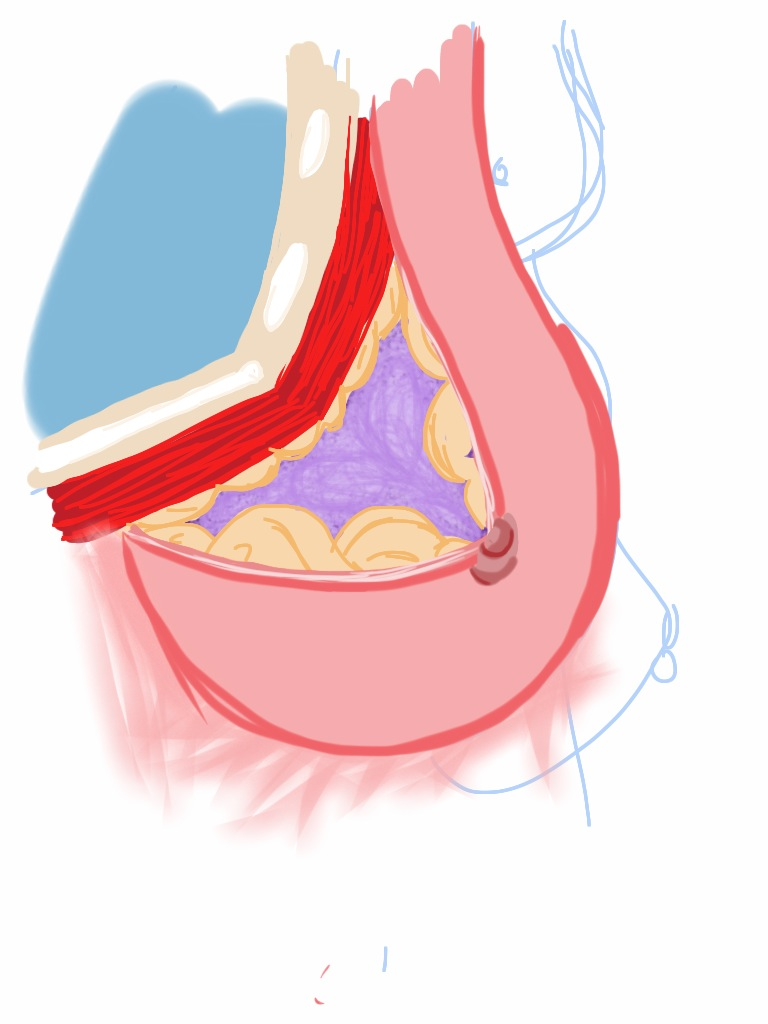
\includegraphics[trim = 20 190 80 20, clip,height=\textwidth]{pit.jpg}};
    \draw		(1.75,	7.75	) 	node[dot]	(AirCoord)			{}	
    				(2.5	,	5		) 	node[dot]	(PecCoord)			{}
    				(3.75,  7.75	) 	node[dot]	(CWCoord)			{}
    				(5,		5.40	) 	node[dot]	(TissueCoord)	{}
    				(2.5	,	3.65	) 	node[dot]	(SkinCoord)		{}
    				(3.75, 3.8	)  	node[dot]	(CooperCoord)	{}
    				(5.80, 5.40	)  	node[dot]	(FatCoord)			{};
 	   				
\draw	(AirCoord)	node[above left] (AirName) {Lungs (air)}
			node[below =of AirName.west, anchor=west] (PecName){Pectoral muscle}
   			(4.5,9.5)	node[anchor=west] (CWName){Chest-wall}
			node[below = of CWName,anchor=west,text width=2cm] (TissueName){Fibro-glandular tissue}
%    			(SkinCoord)
    			node[below= 1.8 of PecName.west, anchor=west ] (SkinName){Skin layers}
    			(CooperCoord |- SkinName)	node[text width=1.5cm,anchor= north west,inner sep=0mm,xshift=-5pt] (CooperName){Cooper's ligament}
    			(FatCoord) node[xshift=9,inner sep=0mm,anchor=west,text width=2cm] (FatName){Adipose tissue \emph{fat lobe}}
;   					 	
    \draw 	(PecCoord) -- (PecName)
    		   	(SkinCoord) -- (SkinName) 
				(CooperCoord) -- (CooperName)
%				(AirCoord) -- (AirName.south)
				(CWCoord) -- (CWName)
				(TissueCoord) -- (TissueName.west)
				(FatCoord) -- (FatName)
				;
%    
%    \draw[help lines,xstep=.5,ystep=.5] (0,0) grid (10,10);
%\foreach \x in {0,1,...,10} { \node [anchor=north] at (\x,0) {\x}; }
%\foreach \y in {0,1,...,10} { \node [anchor=east] at (0,\y) {\y}; });
\end{scriptsize}
\end{tikzpicture}
		\caption{Breast structure elements.}
		\end{figure}	
\end{column}

\begin{column}{.48\textwidth}
\begin{overprint}
\onslide<1|handout:0>
\begin{figure}
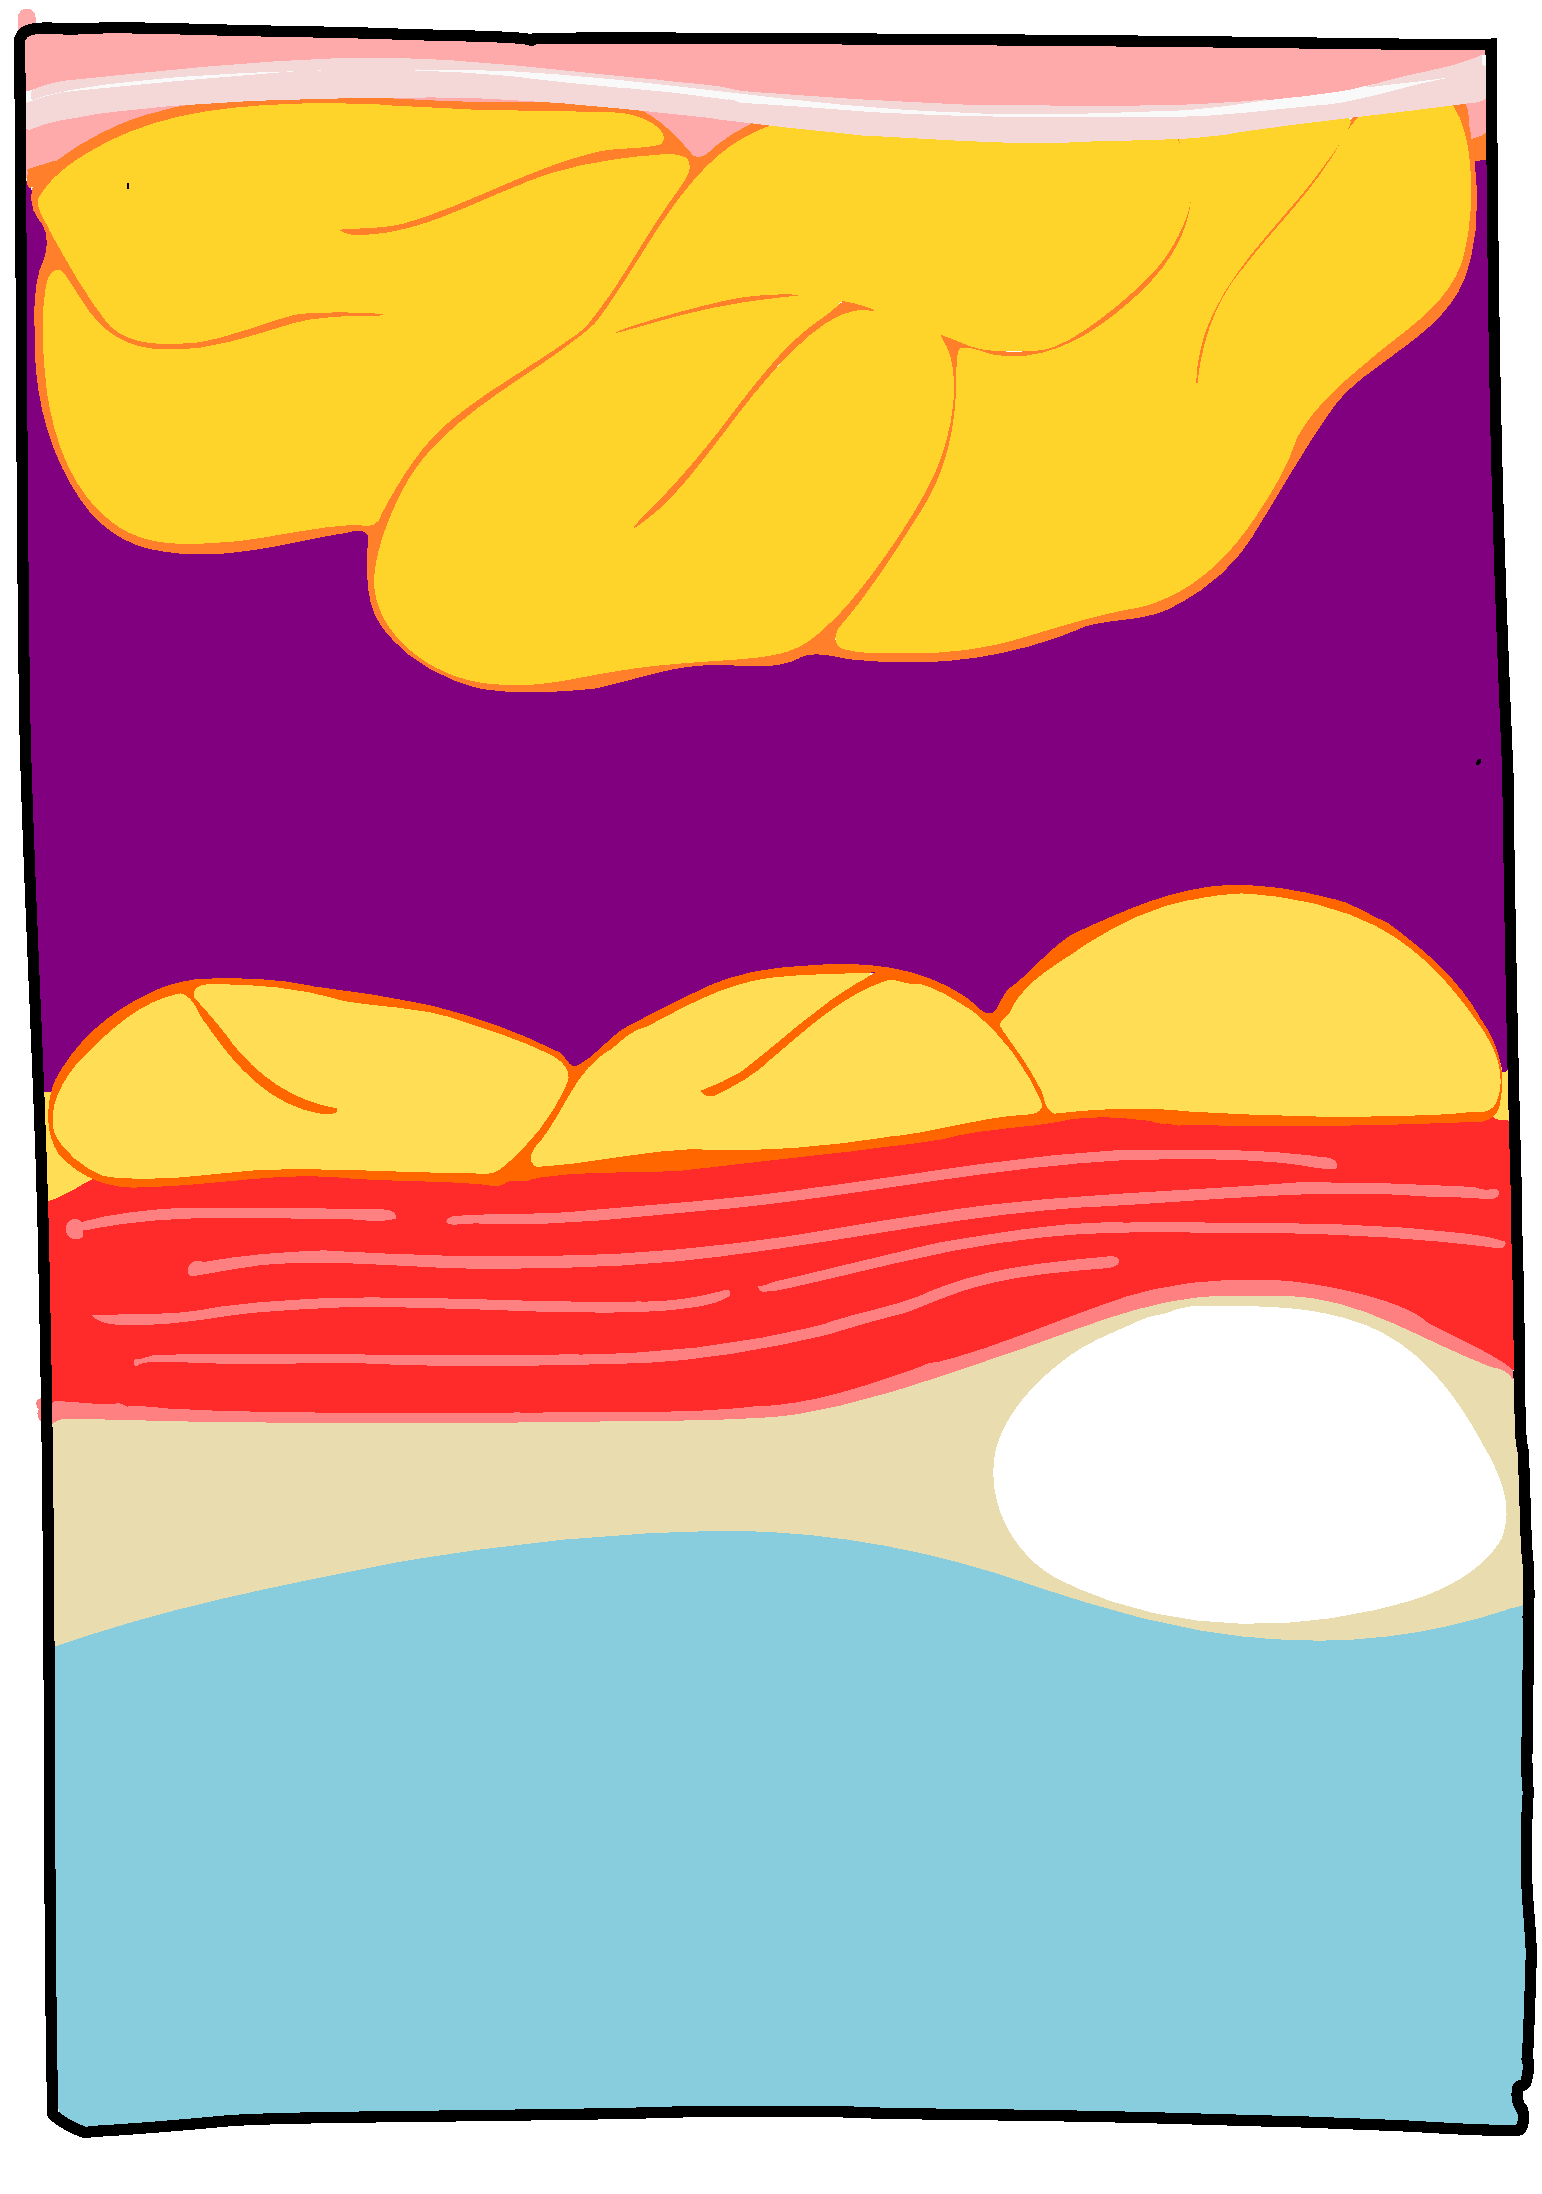
\includegraphics[width=.7\textwidth]{slice/tissue.pdf}
\caption{ Scheme of the elements present in a Breast \ac{us} image.}
		\end{figure}	
		
\onslide<2|handout:0>
		\begin{figure}
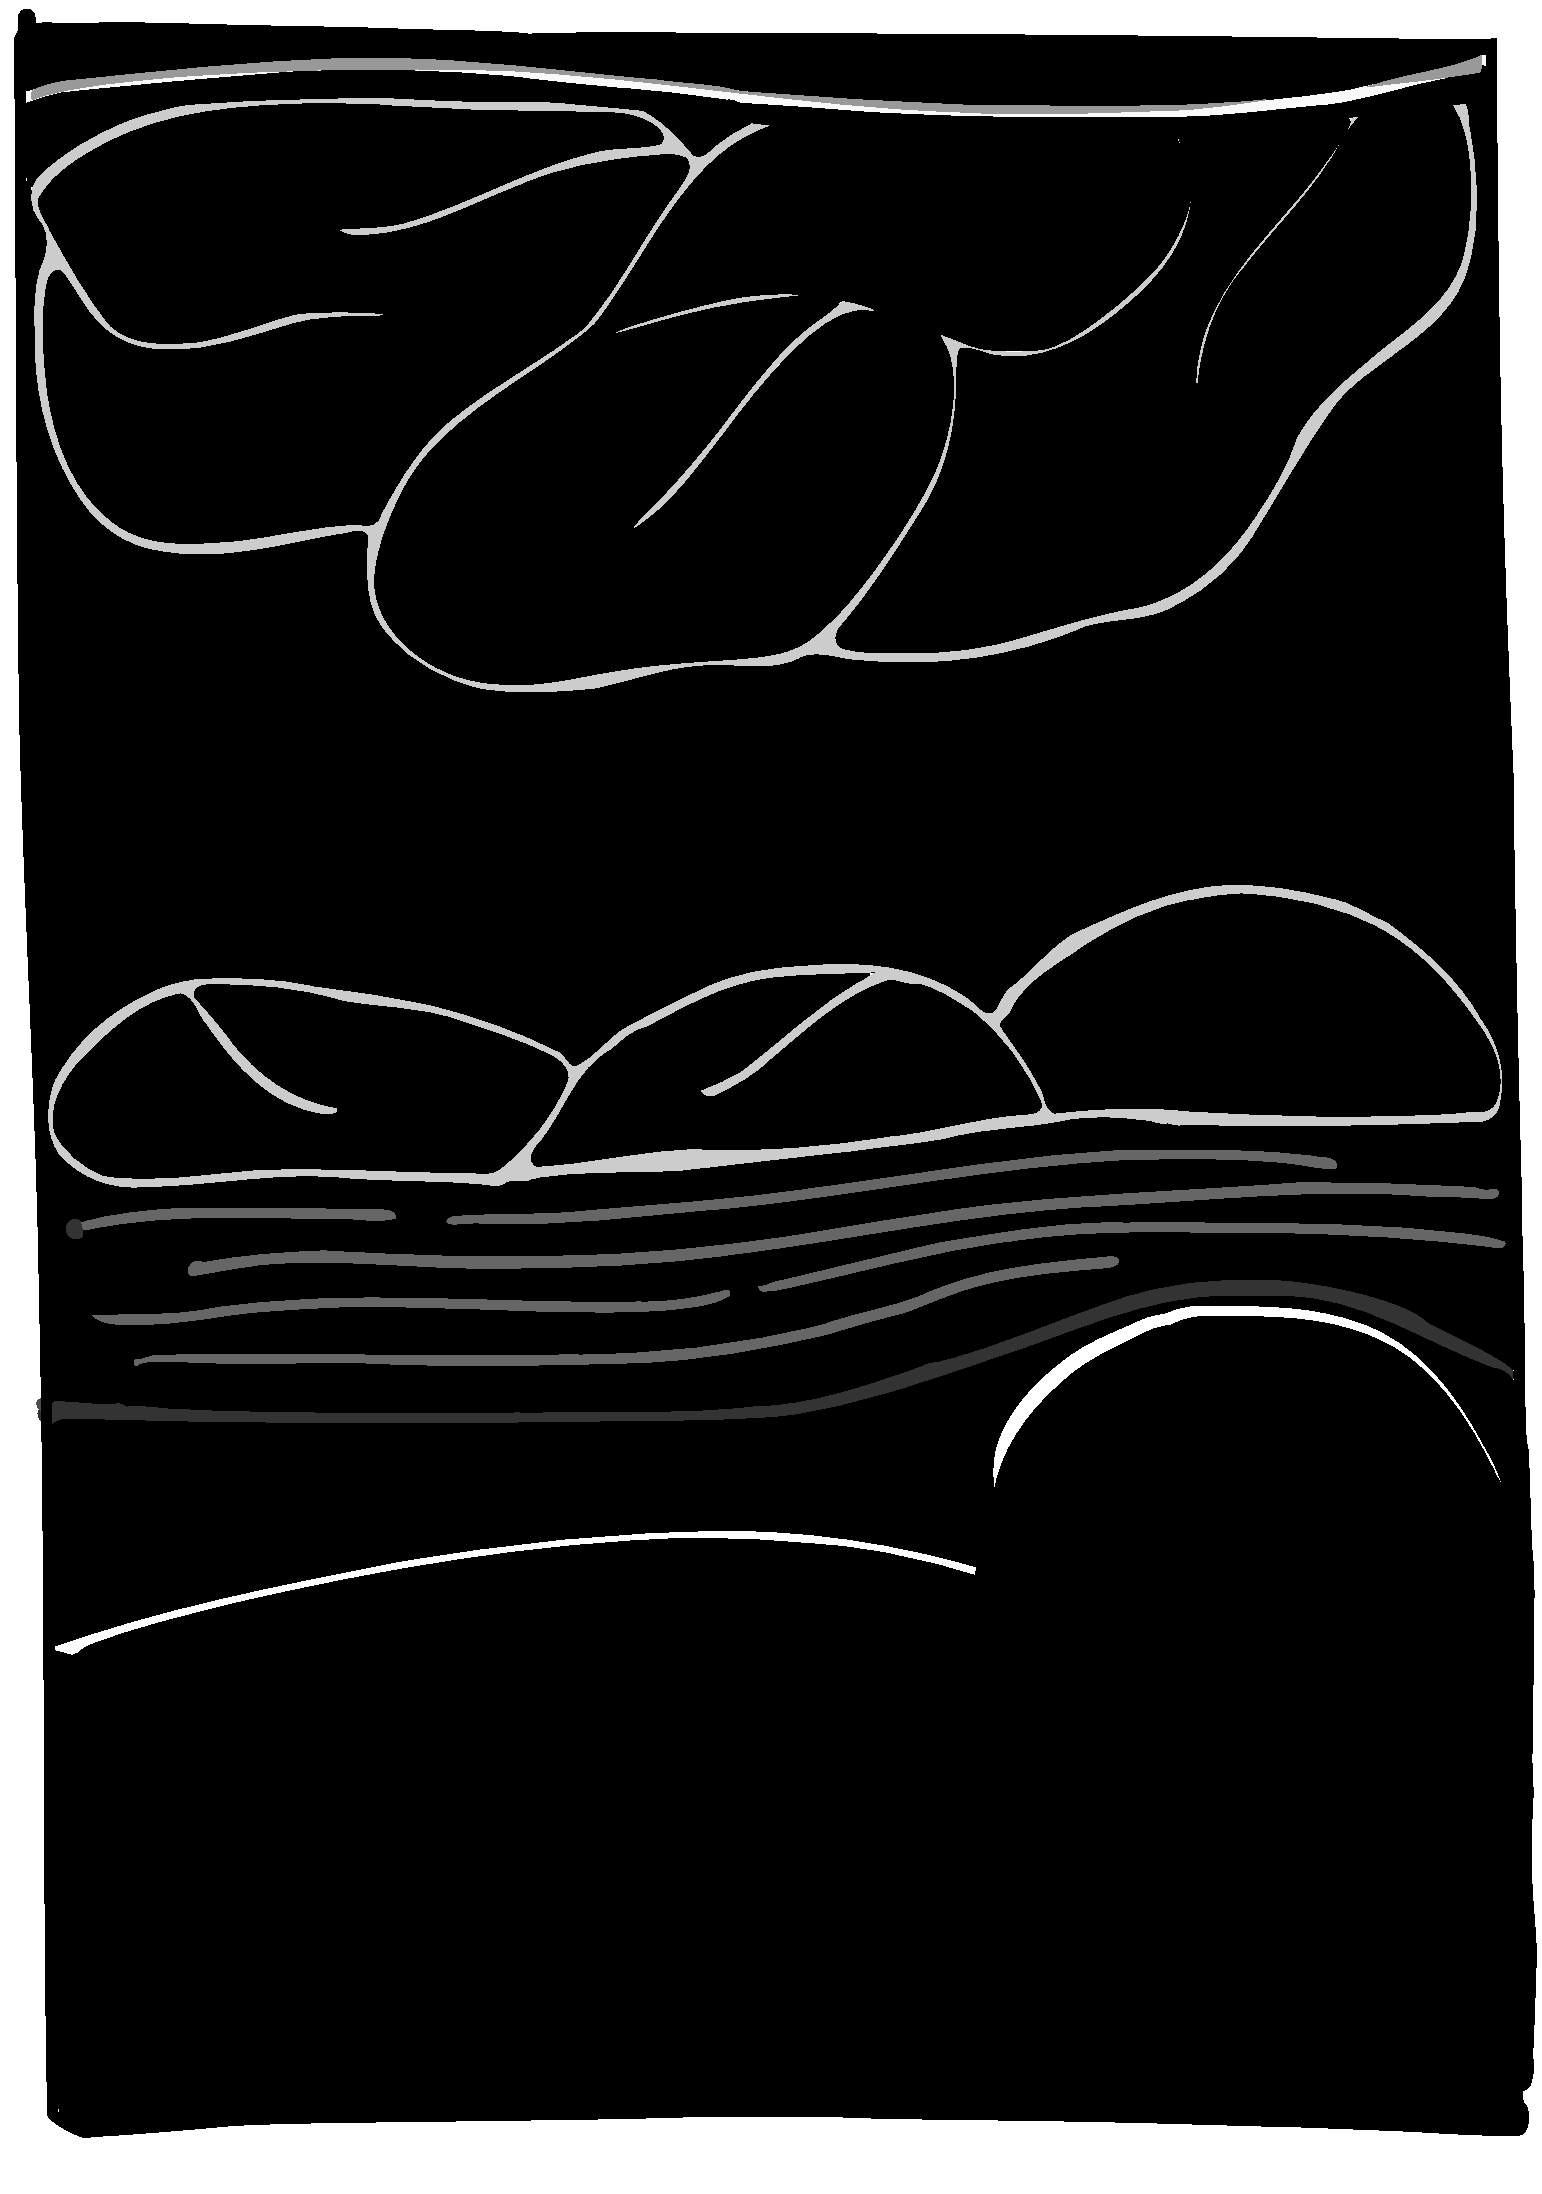
\includegraphics[width=.7\textwidth]{slice/US.pdf}
	\caption{Ideal Breast \ac{us} screening based on depicting the reflection produced on the different tissue boundaries.}
		\end{figure}	
\end{overprint}
\end{column}
\end{columns}
\end{frame}

\begin{frame}\frametitle{Breast structures and appearance under US screening}
%This slide needs to be parted into two slides or a dinamic one where first is olny analyzed specular reflection and seond the scattering.
\begin{columns}
\begin{column}{.48\textwidth}\hspace{-1cm}
\begin{tikzpicture}[scale=1]
\begin{scriptsize}
	 \node[anchor=south west,inner sep=0] at (0,0) {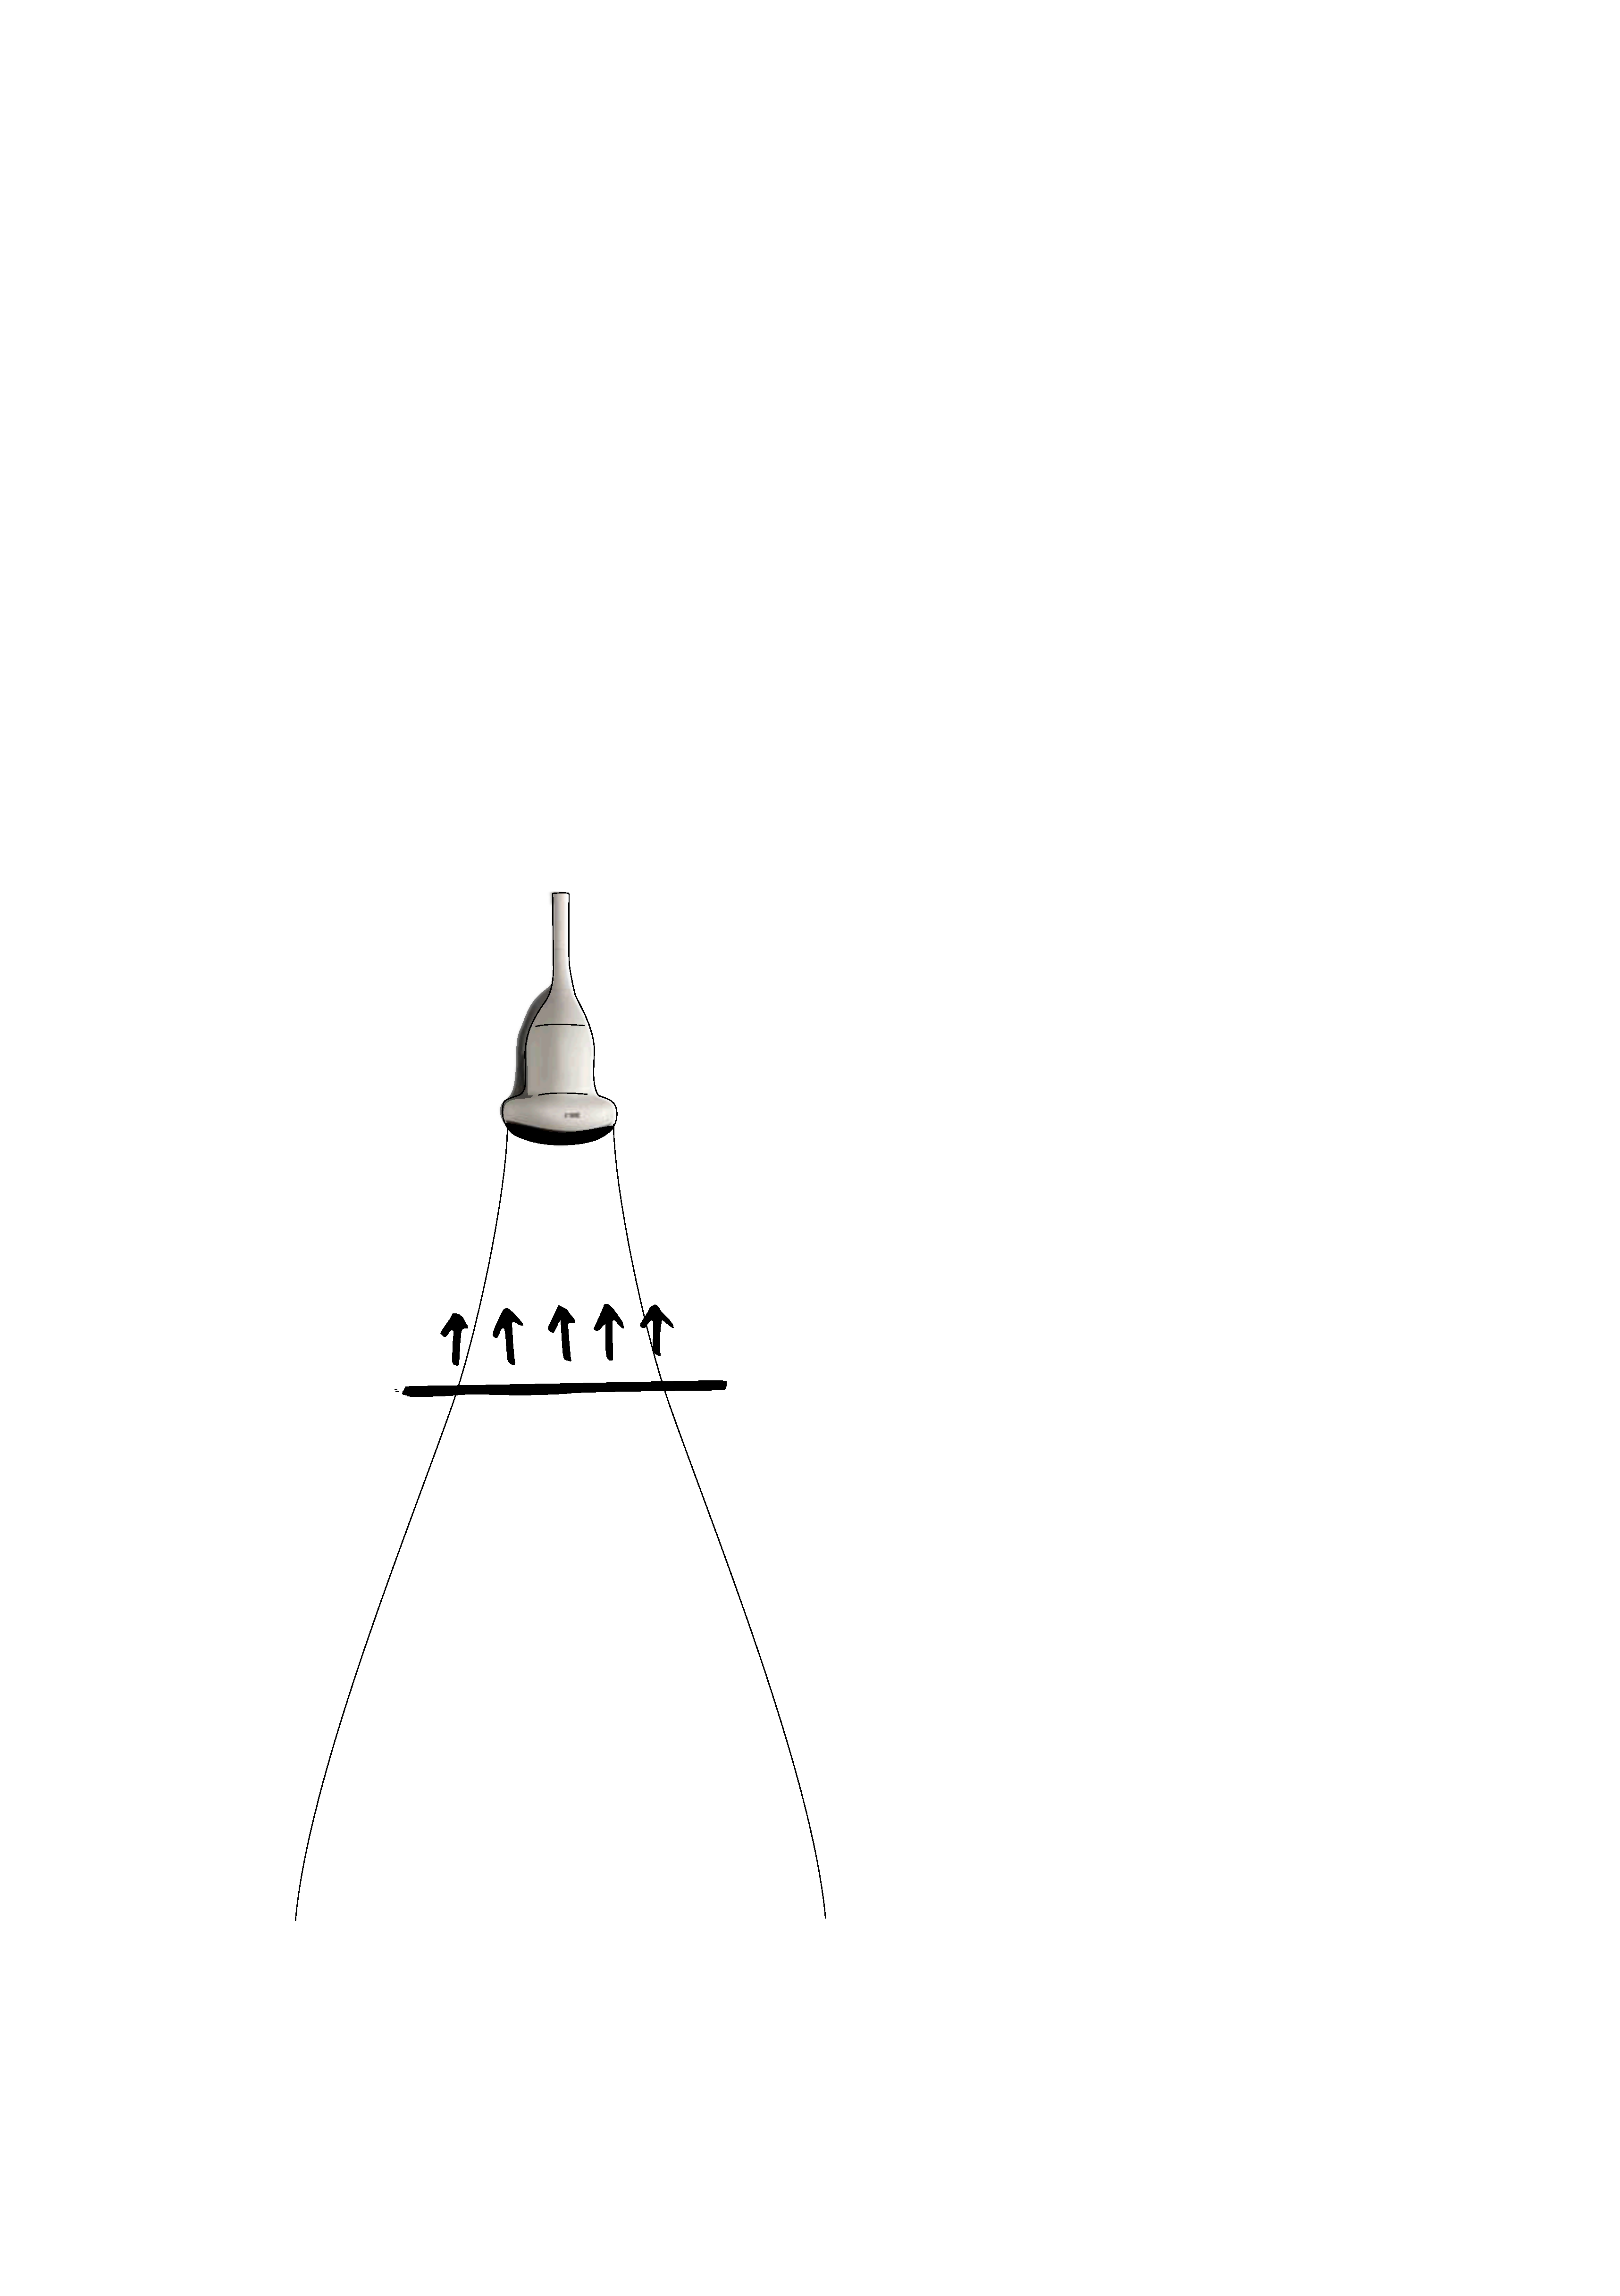
\includegraphics[trim = 300 350 800 1000, clip,width=.8\textwidth]{USscattering/master2.pdf}};
 
%    \draw[help lines,xstep=.5,ystep=.5] (0,0) grid (4,8);
%\foreach \x in {0,.5,1,...,4} { \node [anchor=north] at (\x,8) {\x}; }
%\foreach \y in {0,.5,1,...,8} { \node [anchor=east] at (0,\y) {\y}; });

\def\waveXCenter{2.1}
\def\waveIni{6.3}
\def\waveFin{1}
\def\waveAmplitud{.8}
  \draw[decorate, decoration={snake, segment length=15, amplitude=15},red] (2.03,6) -- (2.03,4.3);
  \draw[decorate, decoration={snake, segment length=15, amplitude=8},red] (2.03,4.3) -- (2.03,.9);
 
\draw 	(0.5,4.7) node[anchor=east] {$R=\frac{Z_2 - Z_1}{Z_2+Z_1}$}
			(0.5,4) node[anchor=east] {$T=\frac{2Z_2}{Z_2+Z_1}$}
			(3.2,4.7) node[anchor=west] {$Z_1$}
			(3.2,4) node[anchor=west] {$Z_2$};

\end{scriptsize}
\end{tikzpicture}
\end{column}

\begin{column}{.48\textwidth}
		\begin{figure}
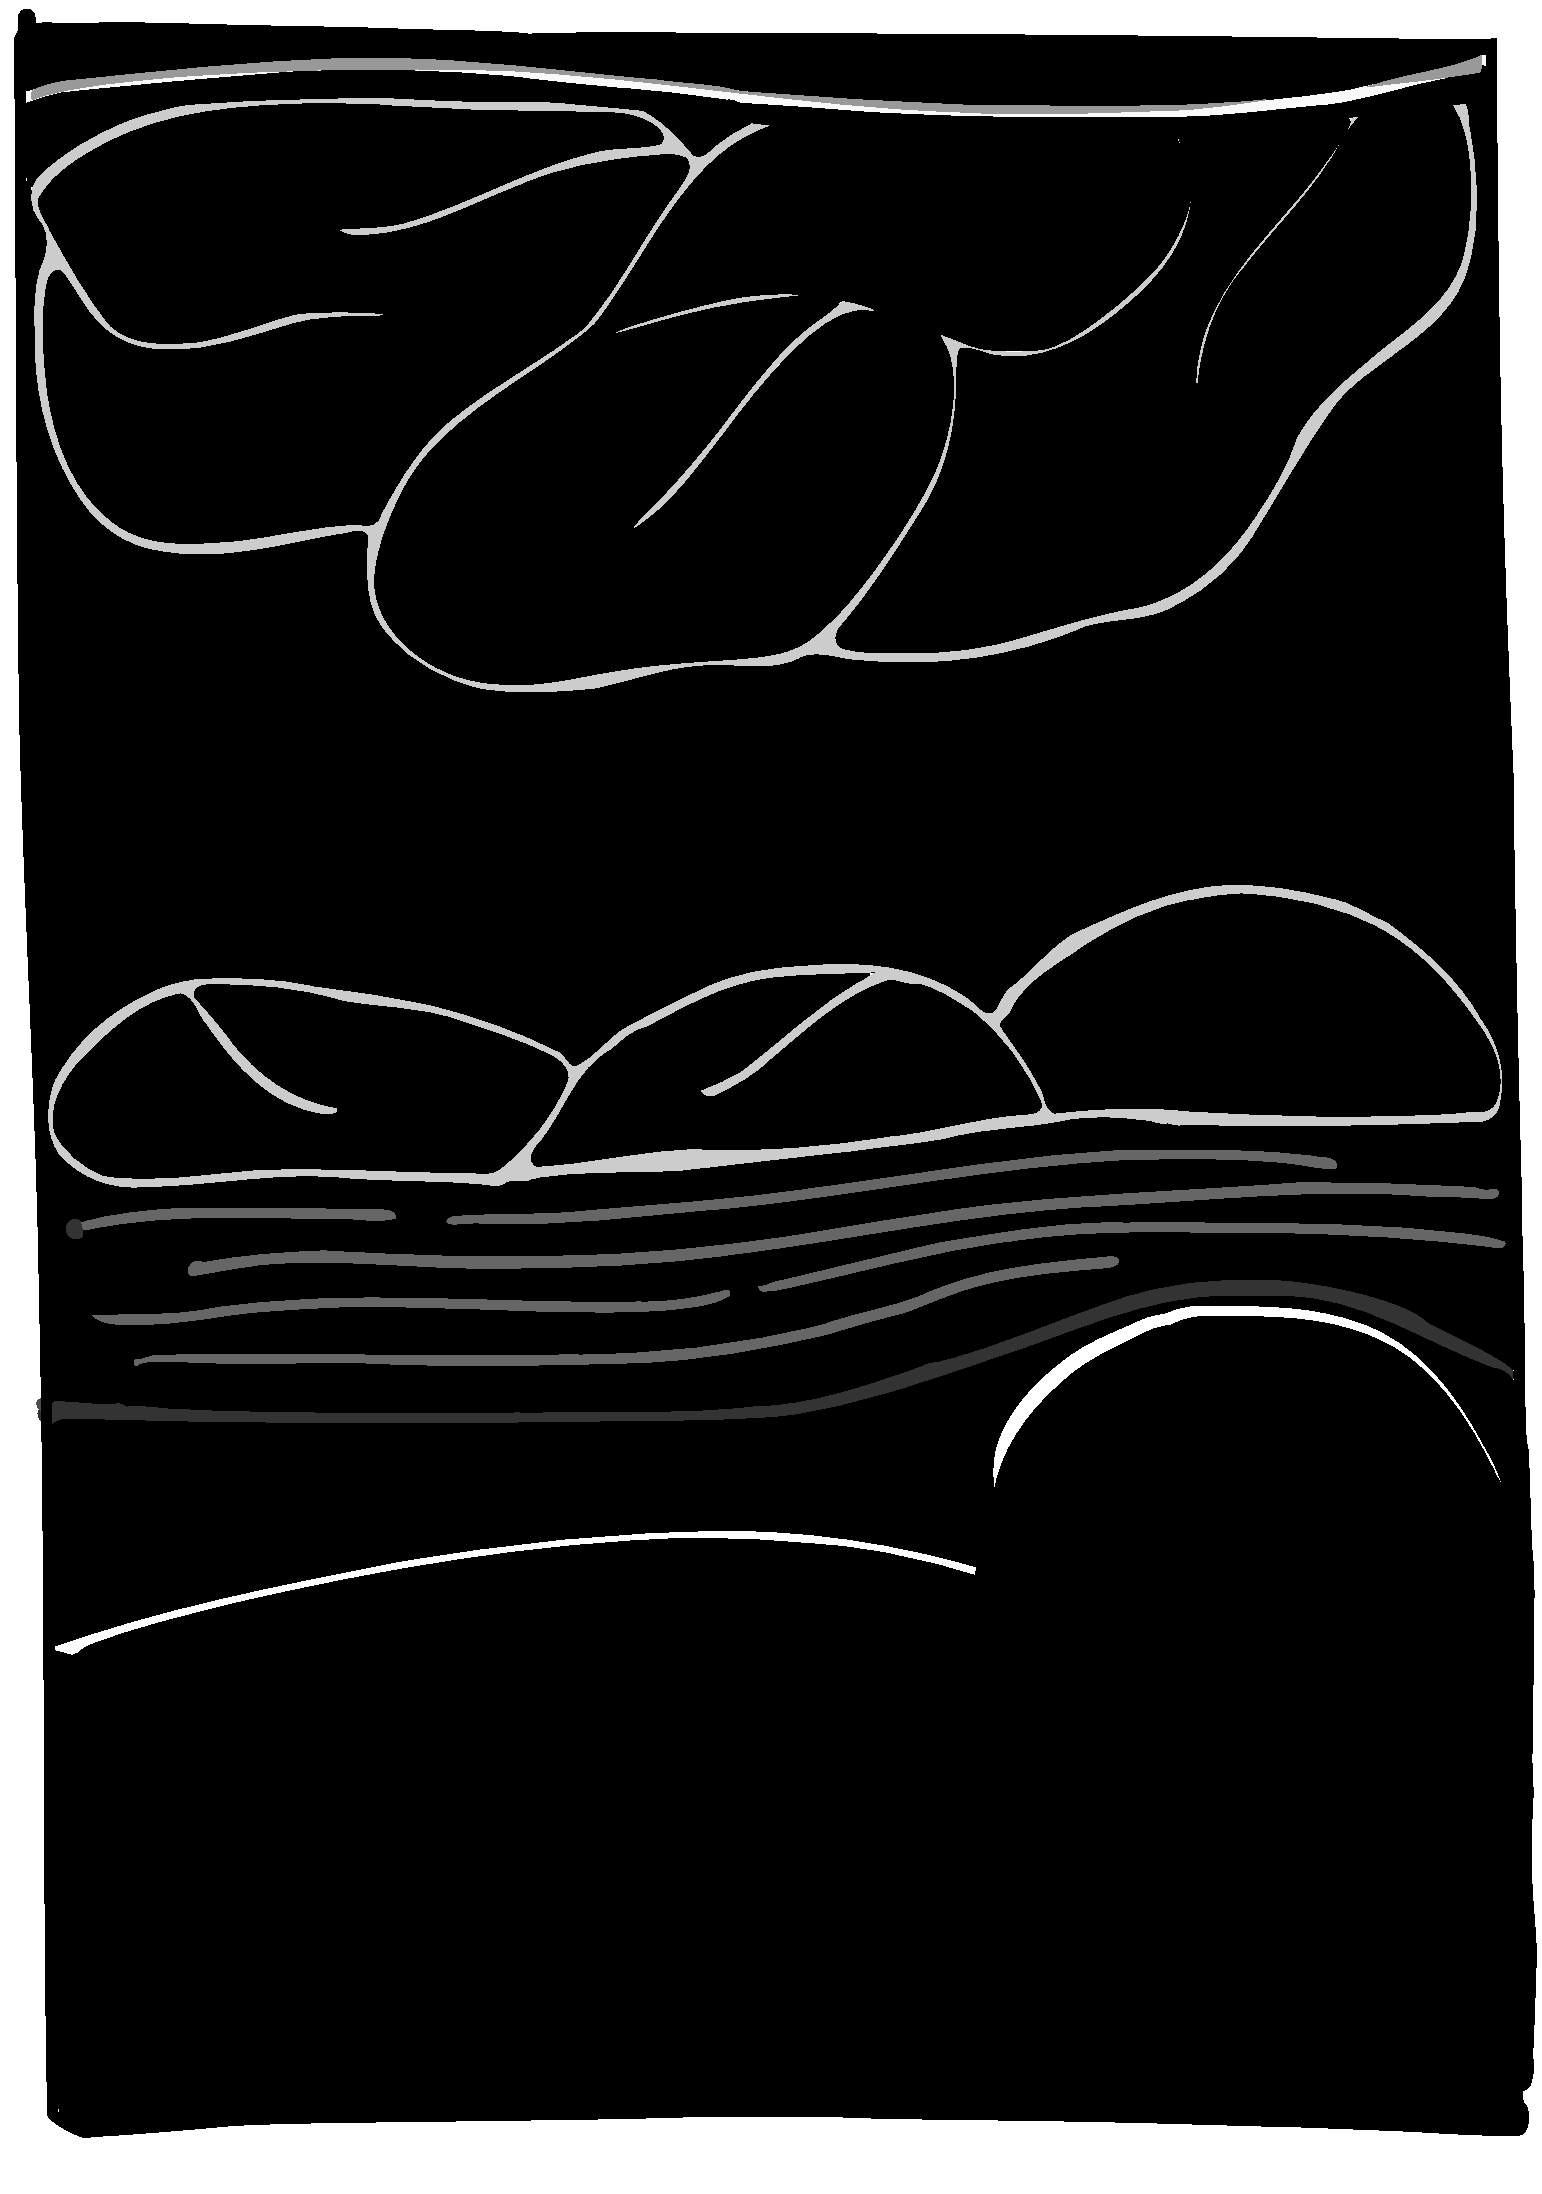
\includegraphics[width=.7\textwidth]{slice/US.pdf}
	\caption{Ideal Breast \ac{us} screening based on the depicting the reflection produced on the different tissue boundaries.}
		\end{figure}
\end{column}
\end{columns}
\end{frame}

\begin{frame}\frametitle{Breast structures and appearance under US screening}
		\begin{figure}
		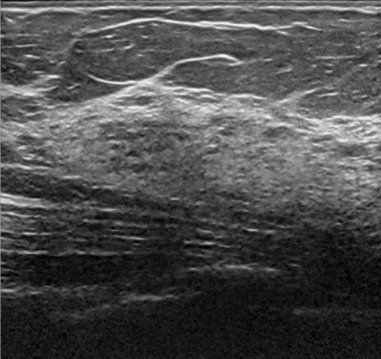
\includegraphics[height=.55\textheight]{sa1.png}~
		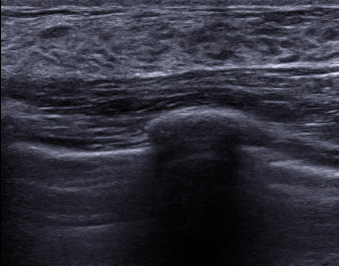
\includegraphics[height=.55\textheight]{sa2.png}
		\caption{ Ultrasound screening examples of two healthy breasts.}
		\end{figure}	
\end{frame}

\subsection{Image inspection to infer state of health}
%\subsection{Computer Aided Diagnosis (CAD)}

\begin{frame}\frametitle{State of health from image visual Inspection}
\setbeamercovered{transparent}
\begin{block}{Radiologic diagnosis error rates are similar to any other human visual inspection\footnotemark[1]}
  \begin{itemize}
    \item Quality of the images.
    \item Ability to interpret the physical properties of the images.
  \end{itemize}
\end{block}
  \begin{enumerate}
    \item <2-> Double readings.
    \item <3-> Utilization of computers to aid the radiologists during the diagnosis process\footnotemark[2]$^,$\footnotemark[3].
  \end{enumerate}
\footnotetext[1]{\fullcite{manning2005perception}}
\onslide<3>
\footnotetext[2]{\fullcite{lusted1955medical}}
%\footnotetext[3]{\fullcite{chan1990improvement}}
\footnotetext[3]{\fullcite{giger2008anniversary}}
\end{frame}


\definecolor{colorTheme}{RGB}{51,41,178}
\begin{frame}\frametitle{\tikz[baseline,inner sep=1.5pt] \node[circle,draw,thick,anchor=base] {1};~Common attributes for describing the image content}
\begin{itemize}
\vspace{-5pt}
\item BKGD Echotexture :
			adipose, fibro-glandular, heterogeneous
\item Mass shape :
	\begin{tikzpicture}[baseline=(label.north)]
	\coordinate (rect) at (.5,.5);
	\coordinate (aux) at (.5,.53);

	\begin{tiny}
		\draw (0,0) rectangle (rect);
		\draw (0.25,0) node[minimum width=1cm,anchor=north](label){Oval};
		\draw [thick,colorTheme!80!white] (0.25,0.25) ellipse ( .2 and .08);
	\end{tiny}
	
	\begin{pgfonlayer}{background}
	\fill [green!30,rounded corners=2pt] ($ (label.west) !.65! (label.south west) $) rectangle (aux -| label.east);
	\end{pgfonlayer}
	\end{tikzpicture}
		\begin{tikzpicture}[baseline=(label.north)]
	\coordinate (rect) at (.5,.5);
	\coordinate (aux) at (.5,.53);

	\begin{tiny}
		\draw (0,0) rectangle (rect);
		\draw (0.25,0) node[minimum width=1cm,anchor=north](label){Round};
%				   (.25,.25) circle[fill,radius=.18,fill=red];
		\draw [thick,colorTheme!80!white]   (.25,.25) circle[radius=.18];
	\end{tiny}
	
	\begin{pgfonlayer}{background}
	\fill [red!30,rounded corners=2pt] ($ (label.west) !.65! (label.south west) $) rectangle (aux -| label.east);
	\end{pgfonlayer}
	\end{tikzpicture} 
		\begin{tikzpicture}[baseline=(label.north)]
	\coordinate (rect) at (.5,.5);
	\coordinate (aux) at (.5,.53);

	\begin{tiny}
		\draw (0,0) rectangle (rect);
		\draw (0.25,0) node[minimum width=1cm,anchor=north](label){Irregular};
		\draw [thick,colorTheme!80!white,rounded corners=2pt]   (.05,.25) -- (.1, .1)  -- (.2,.3) -- (.3,.2)  -- (.2,.05) -- (.35,.06) -- (.45,.25) -- (.4,.46) -- (.15,.3) -- (.1,.45) -- cycle;		
	\end{tiny}
	
	\begin{pgfonlayer}{background}
	\fill [red!30,rounded corners=2pt] ($ (label.west) !.65! (label.south west) $) rectangle (aux -| label.east);
	\end{pgfonlayer}
	\end{tikzpicture}
		\begin{tikzpicture}[baseline=(label.north)]
	\coordinate (rect) at (.5,.5);
	\coordinate (aux) at (.5,.53);

	\begin{tiny}
		\draw (0,0) rectangle (rect);
		\draw (0.25,0) node[minimum width=1cm,anchor=north](label){Lobular};
		\draw [thick,colorTheme!80!white,rounded corners=2pt]   (.05,.25) -- (.18,.15) -- (.25,.25) -- (.35,.15) -- (.45,.25) -- (.35,.35) -- (.25,.25) -- (.18,.35) -- cycle;
	\end{tiny}
	
	\begin{pgfonlayer}{background}
	\fill [orange!30,rounded corners=2pt] ($ (label.west) !.65! (label.south west) $) rectangle (aux -| label.east);
	\end{pgfonlayer}
	\end{tikzpicture}
\item Mass orientation :
		\begin{tikzpicture}[baseline=(label.north)]
	\coordinate (rect) at (.5,.5);
	\coordinate (aux) at (.5,.53);

	\begin{tiny}
		\draw (0,0) rectangle (rect);
		\draw (0.25,0) node[minimum width=1cm,anchor=north](label){Parallel};
		\draw[gray] (0,.44) -- (.5,.44);
		\draw[gray] (0,.47) -- (.5,.47);
		\draw [thick,colorTheme!80!white] (0.25,0.25) ellipse ( .15 and .06);
	\end{tiny}
	
	\begin{pgfonlayer}{background}
	\fill [green!30,rounded corners=2pt] ($ (label.west) !.65! (label.south west) $) rectangle (aux -| label.east);
	\end{pgfonlayer}
	\end{tikzpicture}
		\begin{tikzpicture}[baseline=(label.north)]
	\coordinate (rect) at (.5,.5);
	\coordinate (aux) at (.5,.53);

	\begin{tiny}
		\draw (0,0) rectangle (rect);
		\draw (0.25,0) node[anchor=north](label){Non-parallel};
		\draw[gray] (0,.44) -- (.5,.44);
		\draw[gray] (0,.47) -- (.5,.47);
		\draw [thick,colorTheme!80!white] (0.25,0.25) ellipse ( .06 and .15);
	\end{tiny}
	
	\begin{pgfonlayer}{background}
	\fill [red!30,rounded corners=2pt] ($ (label.west) !.65! (label.south west) $) rectangle (aux -| label.east);
	\end{pgfonlayer}
	\end{tikzpicture}
\item Mass margin :
		\begin{tikzpicture}[baseline=(label.north)]
	\coordinate (rect) at (.5,.5);
	\coordinate (aux) at (.5,.53);

	\begin{tiny}
		%\draw (0,0) rectangle (rect);
		\node[inner sep=0pt,anchor=south west]  at (0,0) {
\includegraphics[height=.5cm]{birads/circumscribed}};
		\draw (0.25,0) node[minimum width=1cm,anchor=north](label){Circumscribed};
	\end{tiny}
	
	\begin{pgfonlayer}{background}
	\fill [green!30,rounded corners=2pt] ($ (label.west) !.65! (label.south west) $) rectangle (aux -| label.east);
	\end{pgfonlayer}
	\end{tikzpicture}
		\begin{tikzpicture}[baseline=(label.north)]
	\coordinate (rect) at (.5,.5);
	\coordinate (aux) at (.5,.53);

	\begin{tiny}
		\node[inner sep=0pt,anchor=south west]  at (0,0) {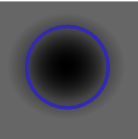
\includegraphics[height=.5cm]{birads/indistinct.png}};
		\draw (0.25,0) node[minimum width=1cm,anchor=north](label){Indistinct};
	\end{tiny}
	
	\begin{pgfonlayer}{background}
	\fill [red!30,rounded corners=2pt] ($ (label.west) !.65! (label.south west) $) rectangle (aux -| label.east);
	\end{pgfonlayer}
	\end{tikzpicture}
		\begin{tikzpicture}[baseline=(label.north)]
	\coordinate (rect) at (.5,.5);
	\coordinate (aux) at (.5,.53);

	\begin{tiny}
		\draw (0,0) rectangle (rect);
		\node[inner sep=0pt,anchor=south west]  at (.03,.12) {
\includegraphics[height=.3cm]{birads/angular}};
		\draw (0.25,0) node[minimum width=1cm,anchor=north](label){Angular};
	\end{tiny}
	
	\begin{pgfonlayer}{background}
	\fill [red!30,rounded corners=2pt] ($ (label.west) !.65! (label.south west) $) rectangle (aux -| label.east);
	\end{pgfonlayer}
	\end{tikzpicture}
		\begin{tikzpicture}[baseline=(label.north)]
	\coordinate (rect) at (.5,.5);
	\coordinate (aux) at (.5,.53);

	\begin{tiny}
			\draw (0,0) rectangle (rect);
		\node[inner sep=0pt,anchor=south west]  at (.05,.12) {
\includegraphics[height=.3cm]{birads/micro.pdf}};
		\draw (0.25,0) node[minimum width=1cm,anchor=north](label){Microlobulated};
	\end{tiny}
	
	\begin{pgfonlayer}{background}
	\fill [red!30,rounded corners=2pt] ($ (label.west) !.65! (label.south west) $) rectangle (aux -| label.east);
	\end{pgfonlayer}
	\end{tikzpicture}
		\begin{tikzpicture}[baseline=(label.north)]
	\coordinate (rect) at (.5,.5);
	\coordinate (aux) at (.5,.53);

	\begin{tiny}
		\draw (0,0) rectangle (rect);
		\node[inner sep=0pt,anchor=south west]  at (0.06,0.1) {
\includegraphics[height=.35cm]{birads/spiculated}};
		\draw (0.25,0) node[minimum width=1cm,anchor=north](label){Spiculated};
	\end{tiny}
	
	\begin{pgfonlayer}{background}
	\fill [red!30,rounded corners=2pt] ($ (label.west) !.65! (label.south west) $) rectangle (aux -| label.east);
	\end{pgfonlayer}
	\end{tikzpicture}
\item Lesion boundary :
		\begin{tikzpicture}[baseline=(label.north)]
	\coordinate (rect) at (.5,.5);
	\coordinate (aux) at (.5,.53);

	\begin{tiny}
%		\draw (0,0) rectangle (rect);
		\node[inner sep=0pt,anchor=south west]  at (0,0) {
\includegraphics[height=.5cm]{birads/Abrupt}};
		\draw (0.25,0) node[minimum width=1cm,anchor=north](label){Abrupt Interface};
	\end{tiny}
	
	\begin{pgfonlayer}{background}
	\fill [green!30,rounded corners=2pt] ($ (label.west) !.65! (label.south west) $) rectangle (aux -| label.east);
	\end{pgfonlayer}
	\end{tikzpicture}
		\begin{tikzpicture}[baseline=(label.north)]
	\coordinate (rect) at (.5,.5);
	\coordinate (aux) at (.5,.53);

	\begin{tiny}
%		\draw (0,0) rectangle (rect);
		\node[inner sep=0pt,anchor=south west]  at (0,0) {
\includegraphics[height=.5cm]{birads/halo}};
		\draw (0.25,0) node[minimum width=1cm,anchor=north](label){Echogenic halo};
	\end{tiny}
	
	\begin{pgfonlayer}{background}
	\fill [red!30,rounded corners=2pt] ($ (label.west) !.65! (label.south west) $) rectangle (aux -| label.east);
	\end{pgfonlayer}
	\end{tikzpicture}
\item Echo pattern :
		\begin{tikzpicture}[baseline=(label.north)]
	\coordinate (rect) at (.5,.5);
	\coordinate (aux) at (.5,.53);

	\begin{tiny}
		\node[inner sep=0pt,anchor=south west]  at (0,0) {
\includegraphics[height=.5cm]{birads/anechoic}};
		\draw (0.25,0) node[minimum width=1cm,anchor=north](label){Anechoic};
	\end{tiny}
	
	\begin{pgfonlayer}{background}
	\fill [green!30,rounded corners=2pt] ($ (label.west) !.65! (label.south west) $) rectangle (aux -| label.east);
	\end{pgfonlayer}
	\end{tikzpicture}
		\begin{tikzpicture}[baseline=(label.north)]
	\coordinate (rect) at (.5,.5);
	\coordinate (aux) at (.5,.53);

	\begin{tiny}
		\node[inner sep=0pt,anchor=south west]  at (0,0) {
\includegraphics[height=.5cm]{birads/hyperechoic}};
		\draw (0.25,0) node[minimum width=1cm,anchor=north](label){Hyperechoic};
	\end{tiny}
	
	\begin{pgfonlayer}{background}
	\fill [green!30,rounded corners=2pt] ($ (label.west) !.65! (label.south west) $) rectangle (aux -| label.east);
	\end{pgfonlayer}
	\end{tikzpicture}
		\begin{tikzpicture}[baseline=(label.north)]
	\coordinate (rect) at (.5,.5);
	\coordinate (aux) at (.5,.53);

	\begin{tiny}
\node[inner sep=0pt,anchor=south west]  at (0,0) {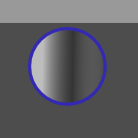
\includegraphics[height=.5cm]{birads/complex.png}};
		\draw (0.25,0) node[minimum width=1cm,anchor=north](label){Complex};
	\end{tiny}
	
	\begin{pgfonlayer}{background}
	\fill [red!30,rounded corners=2pt] ($ (label.west) !.65! (label.south west) $) rectangle (aux -| label.east);
	\end{pgfonlayer}
	\end{tikzpicture}
		\begin{tikzpicture}[baseline=(label.north)]
	\coordinate (rect) at (.5,.5);
	\coordinate (aux) at (.5,.53);

	\begin{tiny}
%		\draw (0,0) rectangle (rect);
		\node[inner sep=0pt,anchor=south west]  at (0,0) {
\includegraphics[height=.5cm]{birads/isoechoic}};
		\draw (0.25,0) node[minimum width=1cm,anchor=north](label){Isoechoic};
	\end{tiny}
	
	\begin{pgfonlayer}{background}
	\fill [orange!30,rounded corners=2pt] ($ (label.west) !.65! (label.south west) $) rectangle (aux -| label.east);
	\end{pgfonlayer}
	\end{tikzpicture}
		\begin{tikzpicture}[baseline=(label.north)]
	\coordinate (rect) at (.5,.5);
	\coordinate (aux) at (.5,.53);

	\begin{tiny}
		\node[inner sep=0pt,anchor=south west]  at (0,0) {
\includegraphics[height=.5cm]{birads/hypoechoic}};
		\draw (0.25,0) node[minimum width=1cm,anchor=north](label){Hypoechoic};
	\end{tiny}
	
	\begin{pgfonlayer}{background}
	\fill [orange!30,rounded corners=2pt] ($ (label.west) !.65! (label.south west) $) rectangle (aux -| label.east);
	\end{pgfonlayer}
	\end{tikzpicture}
\item Posterior acoustic pattern : 
		\begin{tikzpicture}[baseline=(label.north)]
	\coordinate (rect) at (.5,.5);
	\coordinate (aux) at (.5,.53);

	\begin{tiny}
\node[inner sep=0pt,anchor=south west]  at (0,0) {
\includegraphics[height=.5cm]{birads/shadow}};
		\draw (0.25,0) node[minimum width=1cm,anchor=north](label){Shadowing};
	\end{tiny}
	
	\begin{pgfonlayer}{background}
	\fill [red!30,rounded corners=2pt] ($ (label.west) !.65! (label.south west) $) rectangle (aux -| label.east);
	\end{pgfonlayer}
	\end{tikzpicture}
		\begin{tikzpicture}[baseline=(label.north)]
	\coordinate (rect) at (.5,.5);
	\coordinate (aux) at (.5,.53);

	\begin{tiny}
\node[inner sep=0pt,anchor=south west]  at (0,0) {
\includegraphics[height=.5cm]{birads/combined}};
		\draw (0.25,0) node[minimum width=1cm,anchor=north](label){Combined};
	\end{tiny}
	
	\begin{pgfonlayer}{background}
	\fill [red!30,rounded corners=2pt] ($ (label.west) !.65! (label.south west) $) rectangle (aux -| label.east);
	\end{pgfonlayer}
	\end{tikzpicture}
		\begin{tikzpicture}[baseline=(label.north)]
	\coordinate (rect) at (.5,.5);
	\coordinate (aux) at (.5,.53);

	\begin{tiny}
\node[inner sep=0pt,anchor=south west]  at (0,0) {
\includegraphics[height=.5cm]{birads/enhance}};
		\draw (0.25,0) node[minimum width=1cm,anchor=north](label){Enhancement};
	\end{tiny}
	
	\begin{pgfonlayer}{background}
	\fill [orange!30,rounded corners=2pt] ($ (label.west) !.65! (label.south west) $) rectangle (aux -| label.east);
	\end{pgfonlayer}
	\end{tikzpicture}
		\begin{tikzpicture}[baseline=(label.north)]
	\coordinate (rect) at (.5,.5);
	\coordinate (aux) at (.5,.53);

	\begin{tiny}
\node[inner sep=0pt,anchor=south west]  at (0,0) {
\includegraphics[height=.5cm]{birads/hypoechoic}};
		\draw (0.25,0) node[minimum width=1cm,anchor=north](label){No pattern};
	\end{tiny}
	
	\begin{pgfonlayer}{background}
	\fill [orange!30,rounded corners=2pt] ($ (label.west) !.65! (label.south west) $) rectangle (aux -| label.east);
	\end{pgfonlayer}
	\end{tikzpicture}
\end{itemize}

\footnotetext{~\tikz[baseline=(x),inner sep=1.5pt] {\coordinate (x) at (0,-3pt); \node[fill=green!30,rounded corners=2pt,anchor=base,minimum size=10pt] {};} benign, \tikz[baseline=(x),inner sep=1.5pt] {\coordinate (x) at (0,-3pt); \node[fill=red!30,rounded corners=2pt,anchor=base,minimum size=10pt] {};} malignant and \tikz[baseline=(x),inner sep=1.5pt] {\coordinate (x) at (0,-3pt); \node[fill=orange!30,rounded corners=2pt,anchor=base,minimum size=10pt] {};} undetermined founds obtained from a compound of medical works\footnotemark[1].}
\footnotetext[1]{\fullcite{raza2010us}}
\end{frame}


\begin{frame}\frametitle{\tikz[baseline,inner sep=1.5pt] \node[circle,draw,thick,anchor=base] {2};~\acf{cad}}
\vspace{-10pt}
\begin{small}
\begin{block}{\acf{cade}}
{\footnotesize
implies that radiologists use computer outputs of the locations of suspect regions, leaving the characterization, diagnosis, and patient management to be done manually.}
\end{block}
\begin{block}{\acf{cadx}}
{\footnotesize
extends the computer analyses to yield output on the characterization of a region or 
lesion, initially located by either a human or a \ac{cade} system.
}
\end{block}
\vspace{-8pt}
\begin{itemize}
\item 
Most of the descriptors used to describe breast lesions in US data for diagnosis purposes are based on lexicon tools\footnotemark[1]$^,$\footnotemark[2].
\end{itemize}
\end{small}
\footnotetext[1]{\fullcite{Cheng:2009p10580}}
\footnotetext[2]{\fullcite{jalalian2012computer}}
\end{frame}

\begin{frame}\frametitle{Take away}
\item BKGD Echotexture :
			adipose, fibro-glandular, heterogeneous
\item Mass shape :
	\begin{tikzpicture}[baseline=(label.north)]
	\coordinate (rect) at (.5,.5);
	\coordinate (aux) at (.5,.53);

	\begin{tiny}
		\draw (0,0) rectangle (rect);
		\draw (0.25,0) node[minimum width=1cm,anchor=north](label){Oval};
		\draw [thick,colorTheme!80!white] (0.25,0.25) ellipse ( .2 and .08);
	\end{tiny}
	
	\begin{pgfonlayer}{background}
	\fill [green!30,rounded corners=2pt] ($ (label.west) !.65! (label.south west) $) rectangle (aux -| label.east);
	\end{pgfonlayer}
	\end{tikzpicture}
		\begin{tikzpicture}[baseline=(label.north)]
	\coordinate (rect) at (.5,.5);
	\coordinate (aux) at (.5,.53);

	\begin{tiny}
		\draw (0,0) rectangle (rect);
		\draw (0.25,0) node[minimum width=1cm,anchor=north](label){Round};
%				   (.25,.25) circle[fill,radius=.18,fill=red];
		\draw [thick,colorTheme!80!white]   (.25,.25) circle[radius=.18];
	\end{tiny}
	
	\begin{pgfonlayer}{background}
	\fill [red!30,rounded corners=2pt] ($ (label.west) !.65! (label.south west) $) rectangle (aux -| label.east);
	\end{pgfonlayer}
	\end{tikzpicture} 
		\begin{tikzpicture}[baseline=(label.north)]
	\coordinate (rect) at (.5,.5);
	\coordinate (aux) at (.5,.53);

	\begin{tiny}
		\draw (0,0) rectangle (rect);
		\draw (0.25,0) node[minimum width=1cm,anchor=north](label){Irregular};
		\draw [thick,colorTheme!80!white,rounded corners=2pt]   (.05,.25) -- (.1, .1)  -- (.2,.3) -- (.3,.2)  -- (.2,.05) -- (.35,.06) -- (.45,.25) -- (.4,.46) -- (.15,.3) -- (.1,.45) -- cycle;		
	\end{tiny}
	
	\begin{pgfonlayer}{background}
	\fill [red!30,rounded corners=2pt] ($ (label.west) !.65! (label.south west) $) rectangle (aux -| label.east);
	\end{pgfonlayer}
	\end{tikzpicture}
		\begin{tikzpicture}[baseline=(label.north)]
	\coordinate (rect) at (.5,.5);
	\coordinate (aux) at (.5,.53);

	\begin{tiny}
		\draw (0,0) rectangle (rect);
		\draw (0.25,0) node[minimum width=1cm,anchor=north](label){Lobular};
		\draw [thick,colorTheme!80!white,rounded corners=2pt]   (.05,.25) -- (.18,.15) -- (.25,.25) -- (.35,.15) -- (.45,.25) -- (.35,.35) -- (.25,.25) -- (.18,.35) -- cycle;
	\end{tiny}
	
	\begin{pgfonlayer}{background}
	\fill [orange!30,rounded corners=2pt] ($ (label.west) !.65! (label.south west) $) rectangle (aux -| label.east);
	\end{pgfonlayer}
	\end{tikzpicture}
\item Mass orientation :
		\begin{tikzpicture}[baseline=(label.north)]
	\coordinate (rect) at (.5,.5);
	\coordinate (aux) at (.5,.53);

	\begin{tiny}
		\draw (0,0) rectangle (rect);
		\draw (0.25,0) node[minimum width=1cm,anchor=north](label){Parallel};
		\draw[gray] (0,.44) -- (.5,.44);
		\draw[gray] (0,.47) -- (.5,.47);
		\draw [thick,colorTheme!80!white] (0.25,0.25) ellipse ( .15 and .06);
	\end{tiny}
	
	\begin{pgfonlayer}{background}
	\fill [green!30,rounded corners=2pt] ($ (label.west) !.65! (label.south west) $) rectangle (aux -| label.east);
	\end{pgfonlayer}
	\end{tikzpicture}
		\begin{tikzpicture}[baseline=(label.north)]
	\coordinate (rect) at (.5,.5);
	\coordinate (aux) at (.5,.53);

	\begin{tiny}
		\draw (0,0) rectangle (rect);
		\draw (0.25,0) node[anchor=north](label){Non-parallel};
		\draw[gray] (0,.44) -- (.5,.44);
		\draw[gray] (0,.47) -- (.5,.47);
		\draw [thick,colorTheme!80!white] (0.25,0.25) ellipse ( .06 and .15);
	\end{tiny}
	
	\begin{pgfonlayer}{background}
	\fill [red!30,rounded corners=2pt] ($ (label.west) !.65! (label.south west) $) rectangle (aux -| label.east);
	\end{pgfonlayer}
	\end{tikzpicture}
\item Mass margin :
		\begin{tikzpicture}[baseline=(label.north)]
	\coordinate (rect) at (.5,.5);
	\coordinate (aux) at (.5,.53);

	\begin{tiny}
		%\draw (0,0) rectangle (rect);
		\node[inner sep=0pt,anchor=south west]  at (0,0) {
\includegraphics[height=.5cm]{birads/circumscribed}};
		\draw (0.25,0) node[minimum width=1cm,anchor=north](label){Circumscribed};
	\end{tiny}
	
	\begin{pgfonlayer}{background}
	\fill [green!30,rounded corners=2pt] ($ (label.west) !.65! (label.south west) $) rectangle (aux -| label.east);
	\end{pgfonlayer}
	\end{tikzpicture}
		\begin{tikzpicture}[baseline=(label.north)]
	\coordinate (rect) at (.5,.5);
	\coordinate (aux) at (.5,.53);

	\begin{tiny}
		\node[inner sep=0pt,anchor=south west]  at (0,0) {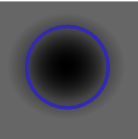
\includegraphics[height=.5cm]{birads/indistinct.png}};
		\draw (0.25,0) node[minimum width=1cm,anchor=north](label){Indistinct};
	\end{tiny}
	
	\begin{pgfonlayer}{background}
	\fill [red!30,rounded corners=2pt] ($ (label.west) !.65! (label.south west) $) rectangle (aux -| label.east);
	\end{pgfonlayer}
	\end{tikzpicture}
		\begin{tikzpicture}[baseline=(label.north)]
	\coordinate (rect) at (.5,.5);
	\coordinate (aux) at (.5,.53);

	\begin{tiny}
		\draw (0,0) rectangle (rect);
		\node[inner sep=0pt,anchor=south west]  at (.03,.12) {
\includegraphics[height=.3cm]{birads/angular}};
		\draw (0.25,0) node[minimum width=1cm,anchor=north](label){Angular};
	\end{tiny}
	
	\begin{pgfonlayer}{background}
	\fill [red!30,rounded corners=2pt] ($ (label.west) !.65! (label.south west) $) rectangle (aux -| label.east);
	\end{pgfonlayer}
	\end{tikzpicture}
		\begin{tikzpicture}[baseline=(label.north)]
	\coordinate (rect) at (.5,.5);
	\coordinate (aux) at (.5,.53);

	\begin{tiny}
			\draw (0,0) rectangle (rect);
		\node[inner sep=0pt,anchor=south west]  at (.05,.12) {
\includegraphics[height=.3cm]{birads/micro.pdf}};
		\draw (0.25,0) node[minimum width=1cm,anchor=north](label){Microlobulated};
	\end{tiny}
	
	\begin{pgfonlayer}{background}
	\fill [red!30,rounded corners=2pt] ($ (label.west) !.65! (label.south west) $) rectangle (aux -| label.east);
	\end{pgfonlayer}
	\end{tikzpicture}
		\begin{tikzpicture}[baseline=(label.north)]
	\coordinate (rect) at (.5,.5);
	\coordinate (aux) at (.5,.53);

	\begin{tiny}
		\draw (0,0) rectangle (rect);
		\node[inner sep=0pt,anchor=south west]  at (0.06,0.1) {
\includegraphics[height=.35cm]{birads/spiculated}};
		\draw (0.25,0) node[minimum width=1cm,anchor=north](label){Spiculated};
	\end{tiny}
	
	\begin{pgfonlayer}{background}
	\fill [red!30,rounded corners=2pt] ($ (label.west) !.65! (label.south west) $) rectangle (aux -| label.east);
	\end{pgfonlayer}
	\end{tikzpicture}
\item Lesion boundary :
		\begin{tikzpicture}[baseline=(label.north)]
	\coordinate (rect) at (.5,.5);
	\coordinate (aux) at (.5,.53);

	\begin{tiny}
%		\draw (0,0) rectangle (rect);
		\node[inner sep=0pt,anchor=south west]  at (0,0) {
\includegraphics[height=.5cm]{birads/Abrupt}};
		\draw (0.25,0) node[minimum width=1cm,anchor=north](label){Abrupt Interface};
	\end{tiny}
	
	\begin{pgfonlayer}{background}
	\fill [green!30,rounded corners=2pt] ($ (label.west) !.65! (label.south west) $) rectangle (aux -| label.east);
	\end{pgfonlayer}
	\end{tikzpicture}
		\begin{tikzpicture}[baseline=(label.north)]
	\coordinate (rect) at (.5,.5);
	\coordinate (aux) at (.5,.53);

	\begin{tiny}
%		\draw (0,0) rectangle (rect);
		\node[inner sep=0pt,anchor=south west]  at (0,0) {
\includegraphics[height=.5cm]{birads/halo}};
		\draw (0.25,0) node[minimum width=1cm,anchor=north](label){Echogenic halo};
	\end{tiny}
	
	\begin{pgfonlayer}{background}
	\fill [red!30,rounded corners=2pt] ($ (label.west) !.65! (label.south west) $) rectangle (aux -| label.east);
	\end{pgfonlayer}
	\end{tikzpicture}
\item Echo pattern :
		\begin{tikzpicture}[baseline=(label.north)]
	\coordinate (rect) at (.5,.5);
	\coordinate (aux) at (.5,.53);

	\begin{tiny}
		\node[inner sep=0pt,anchor=south west]  at (0,0) {
\includegraphics[height=.5cm]{birads/anechoic}};
		\draw (0.25,0) node[minimum width=1cm,anchor=north](label){Anechoic};
	\end{tiny}
	
	\begin{pgfonlayer}{background}
	\fill [green!30,rounded corners=2pt] ($ (label.west) !.65! (label.south west) $) rectangle (aux -| label.east);
	\end{pgfonlayer}
	\end{tikzpicture}
		\begin{tikzpicture}[baseline=(label.north)]
	\coordinate (rect) at (.5,.5);
	\coordinate (aux) at (.5,.53);

	\begin{tiny}
		\node[inner sep=0pt,anchor=south west]  at (0,0) {
\includegraphics[height=.5cm]{birads/hyperechoic}};
		\draw (0.25,0) node[minimum width=1cm,anchor=north](label){Hyperechoic};
	\end{tiny}
	
	\begin{pgfonlayer}{background}
	\fill [green!30,rounded corners=2pt] ($ (label.west) !.65! (label.south west) $) rectangle (aux -| label.east);
	\end{pgfonlayer}
	\end{tikzpicture}
		\begin{tikzpicture}[baseline=(label.north)]
	\coordinate (rect) at (.5,.5);
	\coordinate (aux) at (.5,.53);

	\begin{tiny}
\node[inner sep=0pt,anchor=south west]  at (0,0) {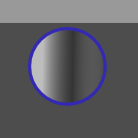
\includegraphics[height=.5cm]{birads/complex.png}};
		\draw (0.25,0) node[minimum width=1cm,anchor=north](label){Complex};
	\end{tiny}
	
	\begin{pgfonlayer}{background}
	\fill [red!30,rounded corners=2pt] ($ (label.west) !.65! (label.south west) $) rectangle (aux -| label.east);
	\end{pgfonlayer}
	\end{tikzpicture}
		\begin{tikzpicture}[baseline=(label.north)]
	\coordinate (rect) at (.5,.5);
	\coordinate (aux) at (.5,.53);

	\begin{tiny}
%		\draw (0,0) rectangle (rect);
		\node[inner sep=0pt,anchor=south west]  at (0,0) {
\includegraphics[height=.5cm]{birads/isoechoic}};
		\draw (0.25,0) node[minimum width=1cm,anchor=north](label){Isoechoic};
	\end{tiny}
	
	\begin{pgfonlayer}{background}
	\fill [orange!30,rounded corners=2pt] ($ (label.west) !.65! (label.south west) $) rectangle (aux -| label.east);
	\end{pgfonlayer}
	\end{tikzpicture}
		\begin{tikzpicture}[baseline=(label.north)]
	\coordinate (rect) at (.5,.5);
	\coordinate (aux) at (.5,.53);

	\begin{tiny}
		\node[inner sep=0pt,anchor=south west]  at (0,0) {
\includegraphics[height=.5cm]{birads/hypoechoic}};
		\draw (0.25,0) node[minimum width=1cm,anchor=north](label){Hypoechoic};
	\end{tiny}
	
	\begin{pgfonlayer}{background}
	\fill [orange!30,rounded corners=2pt] ($ (label.west) !.65! (label.south west) $) rectangle (aux -| label.east);
	\end{pgfonlayer}
	\end{tikzpicture}
\item Posterior acoustic pattern : 
		\begin{tikzpicture}[baseline=(label.north)]
	\coordinate (rect) at (.5,.5);
	\coordinate (aux) at (.5,.53);

	\begin{tiny}
\node[inner sep=0pt,anchor=south west]  at (0,0) {\includegraphics[height=.5cm]{birads/shadow}};
		\draw (0.25,0) node[minimum width=1cm,anchor=north](label){Shadowing};
	\end{tiny}
	
	\begin{pgfonlayer}{background}
	\fill [red!30,rounded corners=2pt] ($ (label.west) !.65! (label.south west) $) rectangle (aux -| label.east);
	\end{pgfonlayer}
	\end{tikzpicture}
		\begin{tikzpicture}[baseline=(label.north)]
	\coordinate (rect) at (.5,.5);
	\coordinate (aux) at (.5,.53);

	\begin{tiny}
\node[inner sep=0pt,anchor=south west]  at (0,0) {\includegraphics[height=.5cm]{birads/combined}};
		\draw (0.25,0) node[minimum width=1cm,anchor=north](label){Combined};
	\end{tiny}
	
	\begin{pgfonlayer}{background}
	\fill [red!30,rounded corners=2pt] ($ (label.west) !.65! (label.south west) $) rectangle (aux -| label.east);
	\end{pgfonlayer}
	\end{tikzpicture}
		\begin{tikzpicture}[baseline=(label.north)]
	\coordinate (rect) at (.5,.5);
	\coordinate (aux) at (.5,.53);

	\begin{tiny}
\node[inner sep=0pt,anchor=south west]  at (0,0) {\includegraphics[height=.5cm]{birads/enhance}};
		\draw (0.25,0) node[minimum width=1cm,anchor=north](label){Enhancement};
	\end{tiny}
	
	\begin{pgfonlayer}{background}
	\fill [orange!30,rounded corners=2pt] ($ (label.west) !.65! (label.south west) $) rectangle (aux -| label.east);
	\end{pgfonlayer}
	\end{tikzpicture}
		\begin{tikzpicture}[baseline=(label.north)]
	\coordinate (rect) at (.5,.5);
	\coordinate (aux) at (.5,.53);

	\begin{tiny}
\node[inner sep=0pt,anchor=south west]  at (0,0) {\includegraphics[height=.5cm]{birads/hypoechoic}};
		\draw (0.25,0) node[minimum width=1cm,anchor=north](label){No pattern};
	\end{tiny}
	
	\begin{pgfonlayer}{background}
	\fill [orange!30,rounded corners=2pt] ($ (label.west) !.65! (label.south west) $) rectangle (aux -| label.east);
	\end{pgfonlayer}
	\end{tikzpicture}
\end{itemize}

\end{frame}

\begin{frame}\frametitle{Wrapping up}
\begin{small}
\begin{itemize}
\item Breast cancer has huge incidence in the population\footnotemark[1].
\item \ac{us} screening is recognized as a useful adjunct image modality\footnotemark[2].
\item Lexicon tools set the standard for breast \ac{us} image reading\footnotemark[3].
\item \ac{cad} systems are proven to help radiologists' to perform more accurate diagnose\footnotemark[4].
\item Reliable \ac{cadx} features are subject to accurate delineation of the lesions\footnotemark[5].
\end{itemize}
\end{small}
\footnotetext[1]{\fullcite{cancerStatistics2011}}
\footnotetext[2]{\vspace{-1pt}\fullcite{smith2003american}}
\footnotetext[3]{\vspace{-1pt}\fullcite{biradsus}}
\footnotetext[4]{\fullcite{giger2008anniversary}}
\footnotetext[5]{\fullcite{jalalian2012computer}}
\end{frame}

\begin{frame}\frametitle{Thesis objective}
\vspace{-5pt}
\begin{block}{Need of accurate delineation of the lesions}
{Development of automatic procedures for segmenting breast lesions in US data.}
\end{block}
\begin{figure}
\includegraphics[trim=0 6 0 0,clip,height=.5\textheight]{a110105_094.png}~
\includegraphics[trim=6 0 0 0,clip,height=.5\textheight]{segment.png}
\caption{Breast \acf{dic} lesion example. Left: original image. Right: several manual delineations generated by 7 different trained experts.}
\end{figure}
\end{frame}


\section{Optimization Based Segmentation}
% \subsection{MRI modalities}

% \setcounter{subfigure}{0}% Reset subfigure counter

% \begin{frame}
%   \frametitle{Introduction}
%   \framesubtitle{MRI modalities}
%   \begin{block}{\small T$_2$W MRI}
%     \begin{figure}%
%       \centering
%       \hspace*{\fill}%
%       \subfigure[][\tiny Healthy]{%
%         \label{fig:t2wh}%
%         \includegraphics[width=.2\textwidth]{./images/mri/t2w/t2w_healthy.eps}}%
%       \hfill%
%       \subfigure[][\tiny CaP PZ]{%
%         \label{fig:t2wcpz}%
%         \includegraphics[width=.2\textwidth]{./images/mri/t2w/t2w_cancer_pz.eps}}%
%       \hfill%
%       \subfigure[][\tiny CaP CG]{%
%         \label{fig:t2wccg}%
%         \includegraphics[width=.2\textwidth]{./images/mri/t2w/t2w_cancer_cg.eps}}%
%       \hspace*{\fill}%
%       \label{fig:t2w}%
%     \end{figure}
%   \end{block}
%   \begin{redblock}{\small Features for CaP}\footnotesize
%     \begin{itemize}
%     \item Low-SI
%     \item Ill-defined shape
%     \end{itemize}
%   \end{redblock}
% \end{frame}

% \setcounter{subfigure}{0}% Reset subfigure counter

% \begin{frame}
%   \frametitle{Introduction}
%   \framesubtitle{MRI modalities}
%   \begin{block}{\small DCE MRI}
%     \begin{figure}%
%       \centering
%       \includegraphics[width=.7\textwidth]{./images/mri/dce/dce_cancer_healthy_information.eps}
%       \label{fig:dce}%
%       \caption{{\color{green}Green}: healthy - {\color{red}Red}: CaP}
%     \end{figure}
%   \end{block}
%   \begin{redblock}{\small Features for CaP}\footnotesize
%     \begin{itemize}
%     \item Faster wash-in, wash-out, time-to-peak enhancement
%     \item Higher integral under the curve, max SI
%     \end{itemize}
%   \end{redblock}
% \end{frame}

% \setcounter{subfigure}{0}% Reset subfigure counter

% \begin{frame}
%   \frametitle{Introduction}
%   \framesubtitle{MRI modalities}
%   \begin{block}{\small DW MRI - ADC}
%     \begin{figure}%
%       \centering
%       \hspace*{\fill}%
%       \subfigure[][\tiny DW MRI]{%
%         \label{fig:dw}%
%         \includegraphics[width=.2\textwidth]{./images/mri/dwi/dwi_cancer.eps}}%
%       \hfill%
%       \subfigure[][\tiny ADC]{%
%         \label{fig:adc}%
%         \includegraphics[width=.2\textwidth]{./images/mri/dwi/adc_cancer.eps}}%
%       \hspace*{\fill}%
%       \label{fig:dwadc}%
%     \end{figure}
%   \end{block}
%   \begin{redblock}{\small Features for CaP}\footnotesize
%     \begin{itemize}
%     \item DW MRI - Higher SI
%     \item ADC - Low-SI
%     \end{itemize}
%   \end{redblock}
% \end{frame}

% \setcounter{subfigure}{0}% Reset subfigure counter

% \begin{frame}
%   \frametitle{Introduction}
%   \framesubtitle{MRI modalities}
%   \begin{block}{\small MRSI}
%     \begin{figure}%
%       \centering
%       \hspace*{\fill}%
%       \subfigure[][\tiny Healthy]{%
%         \label{fig:mrsih}%
%         \includegraphics[width=.45\textwidth]{./images/mri/mrsi/mrsi_healthy.eps}}%
%       \hfill%
%       \subfigure[][\tiny CaP]{%
%         \label{fig:mrsic}%
%         \includegraphics[width=.45\textwidth]{./images/mri/mrsi/mrsi_cancer.eps}}%
%       \hspace*{\fill}%
%       \label{fig:mrsi}%
%     \end{figure}
%   \end{block}
%   \begin{redblock}{\small Features for CaP}\footnotesize
%     \begin{itemize}
%     \item Decrease of citrate and spermine
%     \item Increase of choline
%     \end{itemize}
%   \end{redblock}
% \end{frame}

% \subsection{The MedIA evil}

% \begin{frame}
%   \frametitle{The Medical Imaging evil}
%   \begin{block}<1->{\small The reasons of a nightmare}\footnotesize
%     \begin{itemize}
%     \item[$\rightarrow$] Multidisciplinary competences: medical doctors vs. computer scientists
%     \end{itemize}
%   \end{block}
%   \begin{redblock}<2->{\small Some examples}\footnotesize
%     \begin{itemize}
%     \item Delay in the data acquisition
%     \item Interest differences between the different core competences
%     \item[$\rightarrow$] Lack of interest
%     \end{itemize}
%   \end{redblock}
%   \begin{greenblock}<3->{\small The keystones needed}\footnotesize
%     \begin{itemize}
%     \item Common datasets
%     \item Algorithms comparisons
%     \item Full benchmarking
%     \end{itemize}
%   \end{greenblock}
% \end{frame}

% \section{I2CVB}

% \subsection{Overview}

% \begin{frame}
%   \frametitle{Overview}
%   \begin{block}{\includegraphics[height=.04\textheight]{./images/i2cvb/i2cvb.pdf}\ Platform}
%     \begin{figure}
%       \centering
%       \includegraphics[width=.8\linewidth]{./images/i2cvb/website.pdf}
%     \end{figure}
%     \begin{itemize}
%     \item Development of a web platform
%     \end{itemize}
%   \end{block}
% \end{frame}

% \begin{frame}
%   \frametitle{Manifesto}
%   \begin{columns}
%     \column{.5\textwidth}
%       \begin{block}{\includegraphics[height=.04\textheight]{./images/i2cvb/i2cvb.pdf}\ Vision}
%         \begin{figure}
%           \centering
%           \includegraphics[height=.15\textheight]{./images/i2cvb/research.pdf}
%         \end{figure}
%         \vskip-4ex
%         \begin{itemize}\tiny
%         \item Democratization of the ability to research
%         \end{itemize}
%         \vskip1ex
%       \end{block}
%       \begin{block}{\includegraphics[height=.04\textheight]{./images/i2cvb/i2cvb.pdf}\ Protagonists}
%         \begin{figure}
%           \centering
%           \includegraphics[height=.15\textheight]{./images/i2cvb/shark.pdf}
%         \end{figure}
%         \vskip-4ex
%         \begin{itemize}\tiny
%         \item Research groups and individuals from all walks of life to shape a transparent community
%         \end{itemize}
%       \end{block}
%     \column{.5\textwidth}
%       \begin{block}{\includegraphics[height=.04\textheight]{./images/i2cvb/i2cvb.pdf}\ Mission}
%         \begin{figure}
%           \centering
%           \includegraphics[height=.15\textheight]{./images/i2cvb/what.pdf}
%         \end{figure}
%         \vskip-4ex
%         \begin{itemize}\tiny
%         \item Open data; evaluation methods; comparison framework; reporting platform
%         \end{itemize}
%       \end{block}
%       \begin{block}{\includegraphics[height=.04\textheight]{./images/i2cvb/i2cvb.pdf}\ Strategy}
%         \begin{figure}
%           \centering
%           \includegraphics[height=.15\textheight]{./images/i2cvb/open.pdf}
%         \end{figure}
%         \vskip-4ex
%         \begin{itemize}\tiny
%         \item Transferring successful practises from Free Software and Quality Management
%         \end{itemize}
%         \vskip1ex
%       \end{block}
%   \end{columns}
% \end{frame}

% \subsection{Prostate dataset}

% \begin{frame}
%   \frametitle{I2CVB}
%   \framesubtitle{Prostate dataset}
%   \begin{block}{\small Multi-parametric MRI}\footnotesize
%     \begin{itemize}
%     \item Cohort of 20 patients
%     \item T$_2$W MRI, DCE MRI \& ADC
%     \item 3 Tesla whole body MRI without endorectal coil
%     \end{itemize}
%   \end{block}
%   \begin{greenblock}{\small Ground-truth}\footnotesize
%     \begin{itemize}
%     \item Delineations: prostate - zones - CaP
%     \item Healthy: 2 \textit{vs.} CaP: \{PZ: 13, CG: 3, PZ + CG: 2 \}
%     \end{itemize}
%   \end{greenblock}
% \end{frame}

% \section{Classification framework}

% \begin{frame}
%   \frametitle{Classification framework}
%   \begin{block}{\small Pre-processing}\footnotesize
%     \begin{itemize}
%     \item Resampling data to T$_2$W MRI dataset
%     \item Balancing data using random sampling without replacement
%     \item[$\rightarrow$] 218,423 voxels
%     \end{itemize}
%   \end{block}
%   \begin{block}{\small Features extraction}\footnotesize
%     \begin{itemize}
%     \item Voxel-based ``$V(\cdot)$'': intensities of T$_2$W~MRI, ADC, DCE~MRI \& zonal information (PZ \textit{vs.} CG)
%     \item 3D-texton-based ``$T(\cdot)$'': ($9 \times 9 \times 3$) intensities of T$_2$W~MRI, ADC, DCE~MRI \& zonal information (PZ \textit{vs.} CG)
%     \end{itemize}
%   \end{block}
%   \begin{block}{\small Features classification}\footnotesize
%     \begin{itemize}
%     \item[$\rightarrow$] Gradient Boosted Trees classifier
%     \end{itemize}
%   \end{block}
% \end{frame}

% \section{Results}

% \subsection{Sensitivity \& specificity}

% \setcounter{subfigure}{0}% Reset subfigure counter

% \begin{frame}
%   \frametitle{Results}
%   \begin{block}{\small Sensitivity \& Specificity}\footnotesize
%     \input{./images/results/figures.tex}
%   \end{block}
% \end{frame}

% \subsection{ROC curves}

% \setcounter{subfigure}{0}% Reset subfigure counter

% \begin{frame}
%   \frametitle{Results}
%   \begin{block}{\small ROC curves}\footnotesize
%         \begin{figure}%
%       \centering
%       \hspace*{\fill}%
%       \subfigure[][\tiny Voxel-based]{%
%         \label{fig:rocv}%
%         \includegraphics[width=.45\textwidth]{./images/results/voxel-roc.eps}}%
%       \hfill%
%       \subfigure[][\tiny 3D-texton-based]{%
%         \label{fig:roct}%
%         \includegraphics[width=.45\textwidth]{./images/results/texton-roc.eps}}%
%       \hspace*{\fill}%
%       \label{fig:roc}%
%     \end{figure}
%   \end{block}
% \end{frame}

% \subsection{Conclusion}

% \begin{frame}
%   \frametitle{Conclusion}
%   \begin{greenblock}{\small Discussions}\footnotesize
%     \begin{itemize}
%     \item DCE~MRI is the most disciminative feature
%     \item Combinations of all the modalities lead to better performance
%     \item 3D-texton and neighbourhood information significantly improve the performace
%     \end{itemize}
%   \end{greenblock}
%   \begin{redblock}{\small Future works}\footnotesize
%     \begin{itemize}
%     \item Normalisation of the data in a patient-based fashion
%     \item Use more complex features
%     \item Perform LOPO cross-validation
%     \item Perform a full benchmark study of the current methods!!!!
%     \end{itemize}
%   \end{redblock}
% \end{frame}


\end{document}
